\documentclass[11pt]{amsart}
\usepackage{geometry}                % See geometry.pdf to learn the layout options. There are lots.
\geometry{letterpaper}                   % ... or a4paper or a5paper or ... 
%\geometry{landscape}                % Activate for for rotated page geometry
%\usepackage[parfill]{parskip}    % Activate to begin paragraphs with an empty line rather than an indent
\usepackage{graphicx}
\usepackage{amssymb}
\usepackage{epstopdf}
\usepackage{amsmath}
\usepackage{tikz}
\usepackage{subcaption}
\usepackage{bm}
\usepackage{setspace} 
\doublespacing
\DeclareGraphicsRule{.tif}{png}{.png}{`convert #1 `dirname #1`/`basename #1 .tif`.png}
\usetikzlibrary{arrows,positioning}
% LB things
\newenvironment{packed_item}{
\begin{itemize}
 \setlength{\itemsep}{0pt}
  \setlength{\parskip}{0pt}
  \setlength{\parsep}{0pt}
}{\end{itemize}}

\newcommand{\Unif}{\text{Unif}}
\newcommand{\Beta}{\text{Beta}}
\newcommand{\Normal}{\text{Normal}}
\newcommand{\Binomial}{\text{Binomial}}
\newcommand{\E}{\mathbb{E}}
 
 




\title{Mechanistic Bayesian Forecasts of COVID19}
\author{Graham Gibson, Nicholas Reich, Laura Balzer, Dan Sheldon}
%\date{}                                           % Activate to display a given date or no date


\begin{document}
\section*{Abstract}

As of August 1st 2020 the Covid-19 pandemic has caused over 4 million infections and over 150,000 deaths in the United States alone. Effective modeling of the course of the pandemic can help assist with public health resource planning, intervention efforts, and vaccine clinical trials. However, data quality during a pandemic suffers from under-reporting, backlog reporting, and limited testing. Classical infectious disease differential equation models, such as the susceptible-exposed-infected-recovered model, do not take these data issues into account. We propose a novel Bayesian compartmental model that allows for non-parametric modeling of non-pharamacuetical interventions, time-varying testing, and joint observations on case counts and deaths. The model has been used to submit forecasts to the Covid-hub repository organized by the Reich Lab. We examine the performance relative to the baseline model in addition to performing a nested model comparison of our extensions to the classic models. We demonstrate a significant gain in both MAE and probabilistic scoring measures when taking into account data quality issues during a real-time pandemic.
%\begin{itemize}
%\item Covid has affected XX people
%\item Forecasts useful for public health resource planning, intervention planning (vaccine trials), and disease burden
%\item Basic Mechanistic Models unable to capture complexities of real world disease epidemics due to 
%\begin{itemize}
%\item Complexities of interventions 
%\item Issues with testing and reporting
%\end{itemize}
%\item We propose a novel forecasting algorithm to overcome 
%\begin{itemize}
%\item Under-reporting of cases
%\item Time-varying interventions
%\end{itemize}
%\item Bayesian end to end estimation using both cases and deaths in numpyro
%\end{itemize}


\maketitle

%\section{}
%\subsection{}

\section{Introduction}

The emergence of COVID-19 in early 2020 in the United States developed into the largest pandemic the country has seen in over a century. As of July 2020, there are over 4 million confirmed infections and over 150,000 deaths due to COVID-19 \cite{dong2020interactive}.  Understanding the future trajectory of the pandemic is crucial for minimizing the impact across the nation in terms of healthcare burden, economic recession, and political stability. Forecasts of incident and cumulative deaths due to COVID may help in resource allocation, vaccine clinical trial planning, and re-opening strategies. Along with non-pharamacutical interventions, forecasts are one of the few public health tools available to help fight the pandemic. Infectious disease forecasting has been demonstrated to benefit public health decision makers during annual influenza outbreaks \cite{lutz2019applying}.  However, many forecasts of seasonal disease, such as influenza, often rely on ample historical data to look for patterns that can be projected forward into the future. In an emerging pandemic situation, models must be able to fit to limited data. The COVID-19 pandemic has seen a resurgence in the use of differential equation models to explain the underlying transmission of a disease through a population. First introduced by  Kermack and McKendrick, the model assumes the each individual is in one of a mutually exclusive set of compartments, typically the susceptible, exposed, infected, and recovered compartment \cite{kermack1927contribution}. The model is specified by setting the rates of flow between compartments. While these models have been used since their inception in the early 20th century, the COVID pandemic represents a unique opportunity to explore their properties in real-time. 
Compartmental models have been used to effectively model and forecast disease in non-pandemic situations. These include complex compartmental models for Influenza forecasting \cite{shaman2012forecasting}\cite{osthus2017forecasting}\cite{ong2010real}, including a retrospective model evaluation of the 1918 Influenza pandemic \cite{hall2007real}. Compartmental models have been used not just in respiratory disease but in Ebola \cite{lekone2006statistical}, Measles \cite{bokler1993chaos}, Dengue \cite{syafruddin2012seir} and a wide variety of other disease.

Compartmental models have also been adopted into a Bayesian framework before, including both stochastic disease dynamics and deterministic dynamics \cite{hotta2010bayesian}\cite{dukic2012tracking}. In fact, non-parametric transmissibility was included in a Bayesian SEIR model to study Ebola by Frasso and Lambert \cite{frasso2016bayesian}. Time-varying transmissibility has also been studied in the frequentist setting \cite{smirnova2019forecasting}. With the outbreak of COVID-19, accounting for testing has become a critical element in using an SEIR model. Lopez et al. used a fixed detection probability to model undiagnosed individuals in Spain and Italy \cite{lopez2020modified}. Many efforts have been made to use SEIR models in forecasting COVID-19 \cite{giordano2020modelling}\cite{yang2020modified} \cite{bertozzi2020challenges}\cite{prem2020effect}.

Emerging pandemics create a unique set of challenges for accurately predicting future deaths. These include, but are not limited to, severe under reporting of cases due to asymptomatic transmission, time-varying testing rates, and both the addition and removal of control measures such as social distancing, lockdown, and mask use. In this work, we introduce a set of extensions to the classic compartmental model that are able to account for the real-world and real-time complexities of infectious disease forecasting during a pandemic. We demonstrate the success of the model in both real-time forecast submissions  as well as an ablation test to demonstrate the additional forecast accuracy of our extensions. In what follows we first describe the available data and forecast submission infrastructure, outline the basic susceptible-exposed-infected-recovered (SEIR) compartment model, describe our extensions for real-world pandemic forecasting, and finally evaluate the model using both real-time evaluation from submissions and a retrospective model component analysis. 


%\begin{itemize}
%
%\item Resource allocation
%\item Intervention Planning
%\item Disease burden
%\end{itemize}
%\item Cite Flu Forecasting
%\item Describe COVID-HUB
%\begin{itemize}
%\item Number of participating teams as evidence of importance
%\item Soliciting forecasts for incident and cumulative deaths
%\end{itemize}
%\item Mechanistic models have been around since K\&K
%\item Demonstrated success in modeling infectious disease 
%\item Since they were developed around the last pandemic their usefulness as applied forecasting models has gone untested
%\item Extensions to basic model needed 
%\begin{itemize}
%\item Observations on cases and deaths
%\item Time-varying detection probability for varied testing
%\item Non-parametric model of interventions
%\item Full Bayesian fitting due to unidentifiability of parameters given only a time series of cases and deaths.
%\end{itemize}
%\item MechBayes outperforms in two settings
%\begin{itemize}
%\item COVID-HUB relative to baseline model 
%\item Ablation test relative to basic SEIR model
%\end{itemize}
%\item We show improvements in MAE and WIS relative to baseline model in both experimental setups
%
%\end{itemize}

\section{Data}
	In this analysis we use confirmed case counts and deaths as reported by the Johns Hopkins University Center for Systems Science and Engineering \cite{dong2020interactive}. This a time series dataset which we truncate to begin March 1st 2020 to April 27th 2020 and captures all 50 states, as well as Guam, Puerto Rico, and American Samoa. As noted in \cite{krantz2020level}, COVID-19 cases are often dramatically under-reported, with reporting rates for the U.S. estimated at 20-30\% \cite{russel2020using}. In addition, there has also been severe temporal variation in the percent of symptomatic cases  \cite{russel2020using}. We can also see relatively regular weekly reporting cycles, with reporting dropping off significantly on the weekends. Example incident death data is show in \ref{fig:data}.
	
In order to organize collaborative efforts across the modeling community, the ReichLab of UMass Amherst has developed the COVID-HUB forecast repository and visualization tool \cite{COVID-HUB}. The COVID-HUB team have been soliciting forecasts for 1-4 week ahead incident and cumulative deaths since the beginning of the April 2020. A COVID-HUB forecast is represented by a set of quantiles for incident and cumulative deaths from 1-4 weeks ahead. 

\begin{equation}
\mathbb{Q} = {.05,.10,....,.90,.95} \cup {.01,.99}
\end{equation}
%\begin{itemize}
%\item We use cases/deaths from JHU
%\item Under-reporting issues
%\item Batch reporting issues
%\item Revision Issues
%\item Weekly cycle issues
%\item High variability in incident data
%\item Ref Figure 1
%\end{itemize}

Forecasts are due on Monday evenings and therefore use the incident data up until the Sunday before. A one-week ahead target corresponds to the following Saturday. A two-week ahead corresponds two the next Saturday and so on. Forecasts are stored in the generic repository Zoltar, which allows teams to access both their model and a baseline model \cite{reich2020zoltar}. Zoltar also scores models according to mean-absolute-error (MAE) and the weighted-interval score (WIS) \cite{bracher2020evaluating}. This allows forecasts to be evaluated both point-wise and probabilistically. 



 \begin{figure}
     \centering
     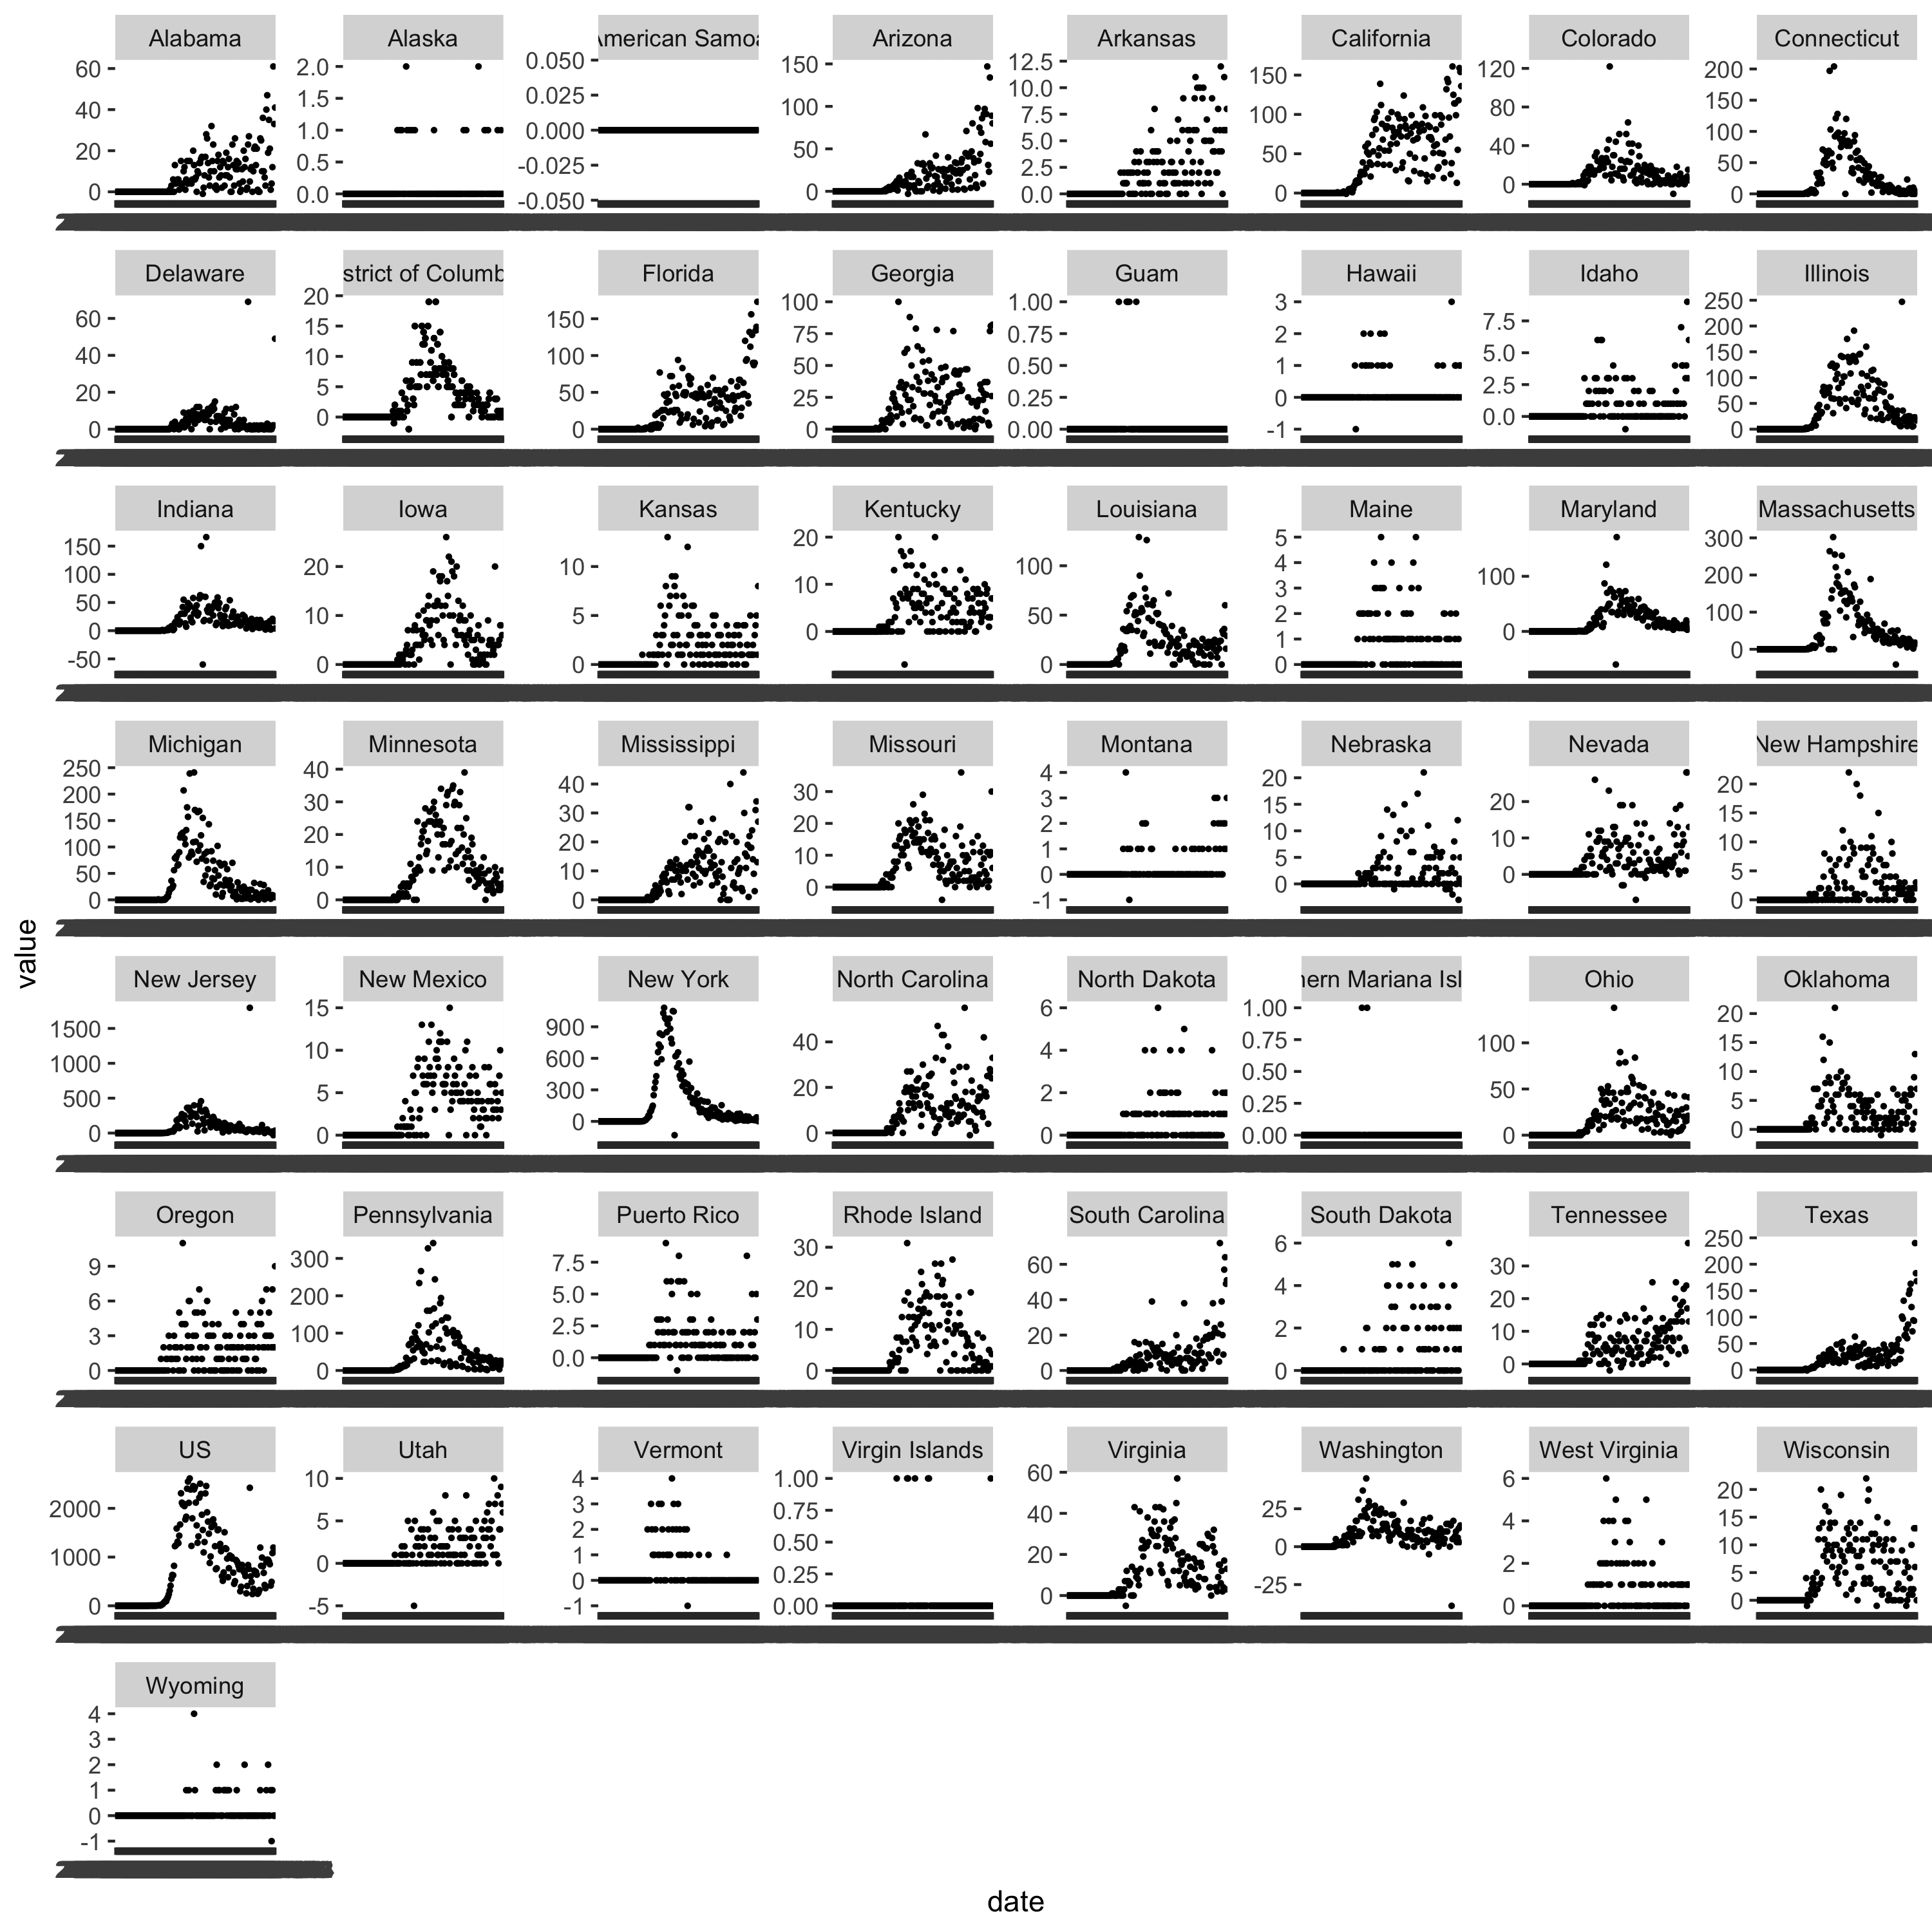
\includegraphics[scale=.175]{data_plot.png}
     \caption{Deaths by state for any state with over 50 incident deaths for a given day. Notice the large variability in incident reporting. There appears to be a weekly cycle where deaths are under-reported on the weekend. We can also see that there are some negative incident deaths, where data are revised to account for deaths that were incorrectly attributed to COVID. }
     \label{fig:data}
 \end{figure}
 
 \section{Compartmental Model}
% \begin{itemize}
% \item Basic SEIR model description
% \item Definition of compartmental model (description of diff eq as flow between compartments)
% \item Ref Figure 2
% \item Interpretation of parameters in basic SEIR model 
% \begin{itemize}
% \item Sigma
% \item Gamma
% \item beta
% \end{itemize}
% 
% \end{itemize}
% 
% \begin{figure}
In a given time-step (e.g. one day), each member of the population of  interest belongs is assumed to be in one of the mutually-and-exhaustive compartments:
 Susceptible $S$, Exposed but not yet infectious $E$, Infectious $I$, Recovered $R$, hospitalized before death $D_1$ , and finally deceased $D_2$. Here we assume everyone who is hospitalized will eventually become deceased in order to separate the rate into both a case fatality ratio (CFR) parameter as well as a time from symptoms to death parameter.    For simplicity, we assume a closed population of size $N$. 
The following parameters govern how members of the population move between compartments:  
\begin{packed_item}
\item $\beta(t)$: transmission rate, which we allow to vary by time $t$
\item $\sigma$: rate of transition from the exposed state $E$ to infectious state $I$; i.e., $1/\sigma$ is the expected duration of the latent period
\item $\gamma$: rate of transition from  the infectious state $I$ to no longer being infectious; i.e., $1/\gamma$ is the expected duration of the infectious period
\item $\rho$: fatality rate %(i.e., probability of transitioning from I to $D_1$ instead of I to R)
\item $\lambda$: rate of transition from $D_1$ to $D_2$ 
(i.e., the inverse of expected number of days in $D_1$ compartment before death) 
\end{packed_item}
For a given time-step $t$, the following differential equations describe the changes in each compartment:
$$\begin{aligned} 
\frac{dS}{dt} &= - \beta(t) \frac{SI}{N} \\
\frac{dE}{dt} &= \beta(t) \cdot \frac{SI}{N} - \sigma E \\
\frac{dI}{dt} &= \sigma E - \gamma I\\ 
\frac{dR}{dt} &= (1-\rho)\gamma I \\
\frac{dD_1}{dt} &= \rho \gamma I - \lambda D_1\\
\frac{dD_2}{dt} &= \lambda D_2\\
\frac{dC}{d} &= \sigma E
\end{aligned} $$


We can write this in a state space representation as follows: \[
X(t) = (S(t), E(t), I(t), R(t), D_1(t), D_2(t))
\]
The update from time $t$ to time $t+1$ can be solved numerically as
$$\bm{X}(t+1)= \text{RK4}\left(\bm{X}(t),\frac{dX}{dt},\beta(t)\right)$$,
where RK4 is the Runge-Katta 4th order approximation (see numpyro ode docs) \cite{numpyro}.


\begin{figure}
 \begin{center}
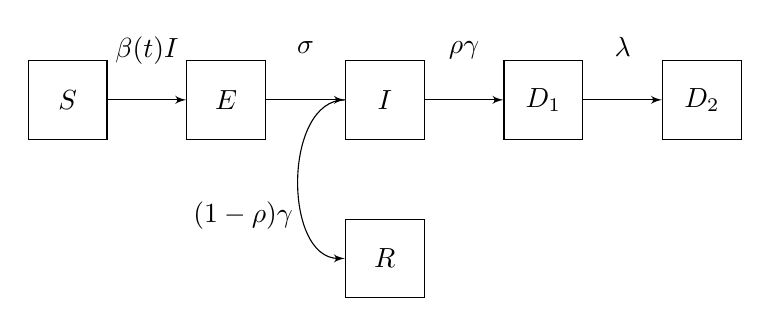
\begin{tikzpicture}[node distance=1cm,auto,>=latex',every node/.append style={align=center},int/.style={draw, minimum size=1cm}]
    \node [int] (S)             {$S$};
      \node [int,right=of S] (E)  {$E$};
    \node [int, right=of E] (I) {$I$};
    \node [int, right=of I] (D_1) {$D_1$};
    \node [int, right=of D_1] (D_2) {$D_2$};
     \node [int, below=of I] (R) {$R$};

   % \coordinate[right=of ] (out); %
    \path[->, auto=false] (S) edge node[yshift=12pt] {$\beta(t) I$ \\[.2em]} (E)
                          (E) edge node[yshift=12pt] {$\sigma$       \\[.2em] } (I) 
                           (I) edge node[yshift=12pt] {$\rho\gamma$       \\[.2em] } (D_1)
                           (I) edge[bend right=90] node[xshift=-20pt,yshift=-20pt] {$(1-\rho)\gamma$       \\[.4em] } (R)
                            (D_1) edge node[yshift=12pt] {$\lambda$       \\[.2em] } (D_2)  ;
                          \end{tikzpicture}
\end{center}
      \caption{Comparmental model parameters }
     \label{fig:seird}
 \end{figure}
 
 
 
 

 
 \subsection{Time-varying transmission parameter}
 
We have seen significant efforts to control the spread of COVID through non-pharmaceutical interventions. These include social distancing, lock-downs, and mask wearing. To add to the complexity, these interventions have been implemented and repealed at different time points. They also face compliance issues. In order to capture the aggregate effect of the interventions non-parametrically we choose a flexible model for the time-varying transmission parameter.
We allow $\beta(t)$ to vary as follows, 

$$log(\beta(t)) \sim N(log(\beta(t-1), \sigma_{\beta}^2)$$

This model assumes that forecasts are made on the current level of interventions. 


% \begin{itemize}
% \item Non-parametrically models time-varying transmissibility through a random walk
% \item Makes forecasts conditional on current level of interventions
% \item Requires no external intervention data to make forecasts 
% \end{itemize}
% 
 \subsection{Observation Model}
 
 The observed data used to fit the model is based on time-series data of confirmed cases $Cases_{t}$ and recorded deaths $Deaths_{t}$. 
For a given state and day, the change in the  confirmed cases and reported deaths are subset of the  number of infections $I(t)$ and underlying number of deaths $D2(t)$, respectively. Therefore, we introduce two additional parameters for the detection probability of cases $p_c$ and the detection probability of deaths $p_d$. For both, we set fairly flat priors to reflect these parameters are poorly determined from observed data.

In more detail, $p_c$ is the probability that an infectious person receives a positive test result and is confirmed as case. We assume its prior distribution is given by  $p \sim \Beta(15, 35)$, such that  $\E[p_c] = 0.3$ with concentration 50. This means that we expect 30\% of cases to be detected initially. However, we also allow this to vary by time.

\begin{equation}
logit(p_{c,t}) \sim N(logit(p_{c,t-1}), \sigma^2)
\end{equation}

We also assume the probability that a COVID-19 death is reported $p_d$ has a prior distribution given by  $p_d \sim \Beta(90, 10)$. This prior satisfies $\E[p_d] = 0.9$ with concentration 100.

 


Using the above SEIR model and these detection probabilities, we can then express the observed numbers of confirmed cases and deaths as follows.
\begin{equation}
\text{Cases}_{t} \sim NB(p_{c,t}*I_{t},\sigma_{c}^2)
\end{equation}

\begin{equation}
\text{Deaths}_{t} \sim NB(p_d*D_{2_{t}}, \sigma_d^2)
\end{equation}


%  \begin{itemize}
% \item Non-parametrically models time varying testing and overall detection of case issues
% \item Allows for "data dumps"
% \item Logistic random walk 
% \item Fixed detection probability on deaths
%
%  \end{itemize}

\subsection{Seeding Epidemic}
Due to the under-reporting of cases, we cannot use the observed data to seed the epidemic. We instead allow the model to find the initial state values for all compartments except the number of susceptible people, which we take as the population size of the geographic region minus the sum of the initial values for the other compartments to enforce the constraint that the entire system size sums to the population size. We do this by assigning uniform probability to all initial states where the number of people in any given compartment at time zero does not exceed 2\% of the total population. This is a highly conservative estimate for the number of infected and exposed people at the start of the epidemic. 


\begin{align*}
 E_0 &\sim \Unif(0, 0.02 N) \\
I_0 &\sim \Unif(0, 0.02 N) \\
  D_{1_0} &\sim \Unif(0, 0.02 N) \\
   D_{2_0} &\sim \Unif(0, 0.02 N) \\   
   R_{0} &\sim \Unif(0, 0.02 N) \\   
\end{align*}

This allows us to initialize the process model:
 $$ X(0) = (S(0), E(0), I(0), R(0), D_1(0), D_2(0), C(0)) = (N-E_0-I_0-D_{1_0}-D_{2_0},E_0,I_0, R_0, D_{1_0}, D_{2_0}, I_0) $$ 
%
% \begin{itemize}
% \item Because of detection probability we cannot seed using initial reported data, since this is an underestimate
% \item Put priors on initial seed
%  \end{itemize}
  
  \subsection{Priors}
We also place the following priors on the transition parameters: 
\begin{align*}
\sigma &\sim \Gamma(5, 5 \hat{d}_E)\\
\gamma & \sim \Gamma(7, 7 \hat{d}_I) \\
\beta(0) &\sim \Gamma(1, \hat{d}_I/\hat{R}) \\
    \rho &\sim \Beta(10, 90)\\ 
\lambda &\sim \Gamma(10, 100)
\end{align*}
 Our prior on rate for leaving the exposed compartment $\sigma$ satisfies $\E[\sigma] = 1/\hat{d}_E$, where $\hat{d}_E$ is an initial guess of the duration of the latent period. Currently, we assume $\hat{d}_E = 4.0$ based on published estimates (shortened slightly to account for possible infectiousness prior to developing symptoms) [cite].
 %
 Our prior on the rate for leaving the infectious compartment $\gamma$ satisfies $\E[\gamma] = 1/\hat{d}_I$, where $\hat{d}_I$ is an initial guess for the duration of infectiousness. The current setting is $\hat{d}_I = 2.0$ to model the likely isolation of individuals after symptom onset (cite). 
Our prior on the initial transmission rate is derived from the relationship between the basic reproductive number $R(0)$ and the length of the infectious period: $R(0) = \beta(0)/\gamma = \beta(0)\times \hat{d}_I$. Therefore, we set our prior on the initial transmission rate to satisfy $\E[\beta(0)] = \hat{R}/\hat{d}_I$ where $\hat{R} = 3.0$ is an initial guess for $R(0)$ and $\hat{d}_I = 2.0$, as described above. 
%%
Our prior on the fatality rate $\rho$ satisfies $\E[\rho] = 0.1$ with concentration of $100$.
Finally, our prior on the rate at which dying patients succumb  satisfies $\lambda$ $\E[\lambda] = 0.1$ with shape 10 corresponding to roughly 10 days in the $D_{1}$ compartment.

The identifiability of model parameters in compartmental models where the data consists of only a time series of incident cases and deaths presents a problem for uninformative priors. Using the renewal style equations, it can be shown that the number of newly infected at time $t$ is a function of the time-varying reproductive number, serial interval and previously reported new infections \cite{wallinga2007generation}. This means that a single time series does not contain enough information to separately estimate both the serial interval and the time-varying reproduction number. In an SEIR model, the serial interval is distributed exponential with rate parameter $\sigma + \gamma$ \cite{wallinga2007generation}. Additionally, the time varying reproduction number is $R_t = \frac{\beta(t)*S(t)}{\gamma}$. Therefore, the time series of incident cases is not enough to uniquely identify $\gamma,\sigma,\beta(t)$. In order to make the model identifiable, we impose tight priors on the parameters $\sigma$ and $\gamma$ as estimated by the literature, in essence fixing the serial interval and we let $\beta(t)$ vary freely. This reflects the underlying biology of the system, since the reciprocal of the sum of $\sigma$ and $\gamma$ may be interpreted as the average time from when an individual becomes infected to when they infect someone else, given that they infect someone else. This is a biological property of the disease, rather than $\beta(t)$ which contains both the biological transmissibility as well as the aggregate effects of human behavior through intervention. This highlights a fundamental philosophical difference between using compartmental models for forecasting rather than interpreting parameters for epidemiological purposes. \textbf{I want to say a little more} 

% \begin{itemize}
% \item We choose tight priors based on literature
%  \item Fundamental unidentifiability due to renewal equation expression where $I(t)$ is a convolution between $R_t$ and Seiral interval
%  \item Cannot estimate both simultaneously 
%  \item Most flexibility comes in with beta and detection random walk
%  \item Ideal for forecasting, maybe not for inference
%  \end{itemize}
%  
  \subsection{Fitting}
We use the hamiltonian monte carlo algorithm implemented in numpyro (some citation here) to fit the model to data. That is, given a time series of confirmed cases ($C_{1:t}$) and confirmed deaths ($D_{1:t}$) we use Bayesian inference (via HMC) to obtain 


$$f(\bm{\theta} | C_{1:t},D_{1:t}) \propto f(C_{1:t},D_{1:t} | \bm{\theta})f(\bm{\theta})$$

where $\bm{\theta}$ is a vector containing all model parameters. 

$$\bm{\theta} =[\beta_{t} ,
\sigma ,
\gamma ,
\rho ,
\lambda ,
p_{c,t} ,
p_{d} ,
\sigma_c^2 ,
\sigma_d^2 ,
I_0 ,
E_0 ,
D_{1_0} ,
D_{2_0} ,
R_0 ]$$


We use the numpyro probabilistic framework to fit the model. 

%
% \begin{itemize}
% \item Fully Bayesian HMC on parameters
% \item Why we choose deterministic compartmental model with only uncertainty on parameters and observations
% \item Estimation in numpyro very fast
%   \end{itemize}
%   
%   
%   
 \section{Experimental Setup}
 To evaluate our model, we examine two different scenarios. First, we describe the submission process and infrastructure used for the real time evaluation as part of the COVID-HUB consortium. Second, we describe the internal evaluation used to demonstrate our model enhancements improve accuracy over a naive compartmental model. 
 
 \subsection{COVID-HUB}
 The COVID-HUB began soliciting forecasts in the beginning of April 2020 for 1-4 week ahead cumulative deaths. We began submitting the first version on April 20th 2020 and have since submitted forecasts every Monday from then until August 1st 2020. The forecasts use daily data up to and including the Sunday before submission the next Monday. The one week ahead forecast corresponds to the following Saturday, the two week ahead to the second following Saturday and so on. Our model went through three distinct iterations as we evaluated performance in real-time. 
 
 \begin{itemize}
 
 \item \textbf{Version 1: April 20th 2020 through May 10th 2020}. Model had normal observation noise (instead of negative binomial) and a non-time varying case detection probability. Model was fit to cumulative deaths. 
  \item \textbf{Version 2: May 10th 2020 through May 24th 2020}. Model had normal observation noise (instead of negative binomial) and time varying case detection probability. Model was fit to cumulative deaths. 
    \item \textbf{Version 3: May 24th 2020 through August 1st 2020}. Model had negative binomial observation noise  and time varying case detection probability. Model was fit to incident deaths. 
 \end{itemize} 
 
 
 These three versions highlight the complexities of forecasting during a real-time pandemic. Models evolve due to real-time evaluations by responding to the unique data collection environments of each pandemic. We use the model submissions made in real-time, under the corresponding version of the model as dated above, evaluated on both MAE and WIS for the weeks of XXXX.
% \begin{itemize}
% \item Real-time forecasting evaluation for 14 weeks starting April 20th 2020. 
% \item Forecasts submitted every Monday using incident data up until Sunday
% \item Cumulative forecasts generated by aggregation of incident forecasts
% \item 1-4 week ahead targets generated from 28 day ahead predictions 
% \end{itemize}
 
 \subsection{Ablation Test}
 
 While real-time model evaluation is valuable for understanding evolving model performance, we also perform a retrospective evaluation using three model variants. We define the following variations on MechBayes,
 
 \begin{itemize}
 \item \textbf{MechBayes Full} Mech Bayes as of model version 3. That is, a model using negative binomial observation noise as well as a time-varying random walk, using a joint likelihood over cases and deaths.
 
 \item \textbf{MechBayes Fixed Case Detection Probability} MechBayes Full with $p_{c,t}$ fixed to $p_c$, that is, removing the time-varying detection probability.
 
 \item \textbf{MechBayes Death Only} MechBayes Full with observations on cases removed.
 \end{itemize}
 
 Note that these are nested models, with MechBayes Death Only contained in MechBayes Fixed Case Detection Probability contained in MechBayes Full. This allows to perform a nested model comparison using MAE as the scoring metric. \textbf{Include something with beta}


\section{COVID-Hub Results}


\begin{figure}
  \centering

    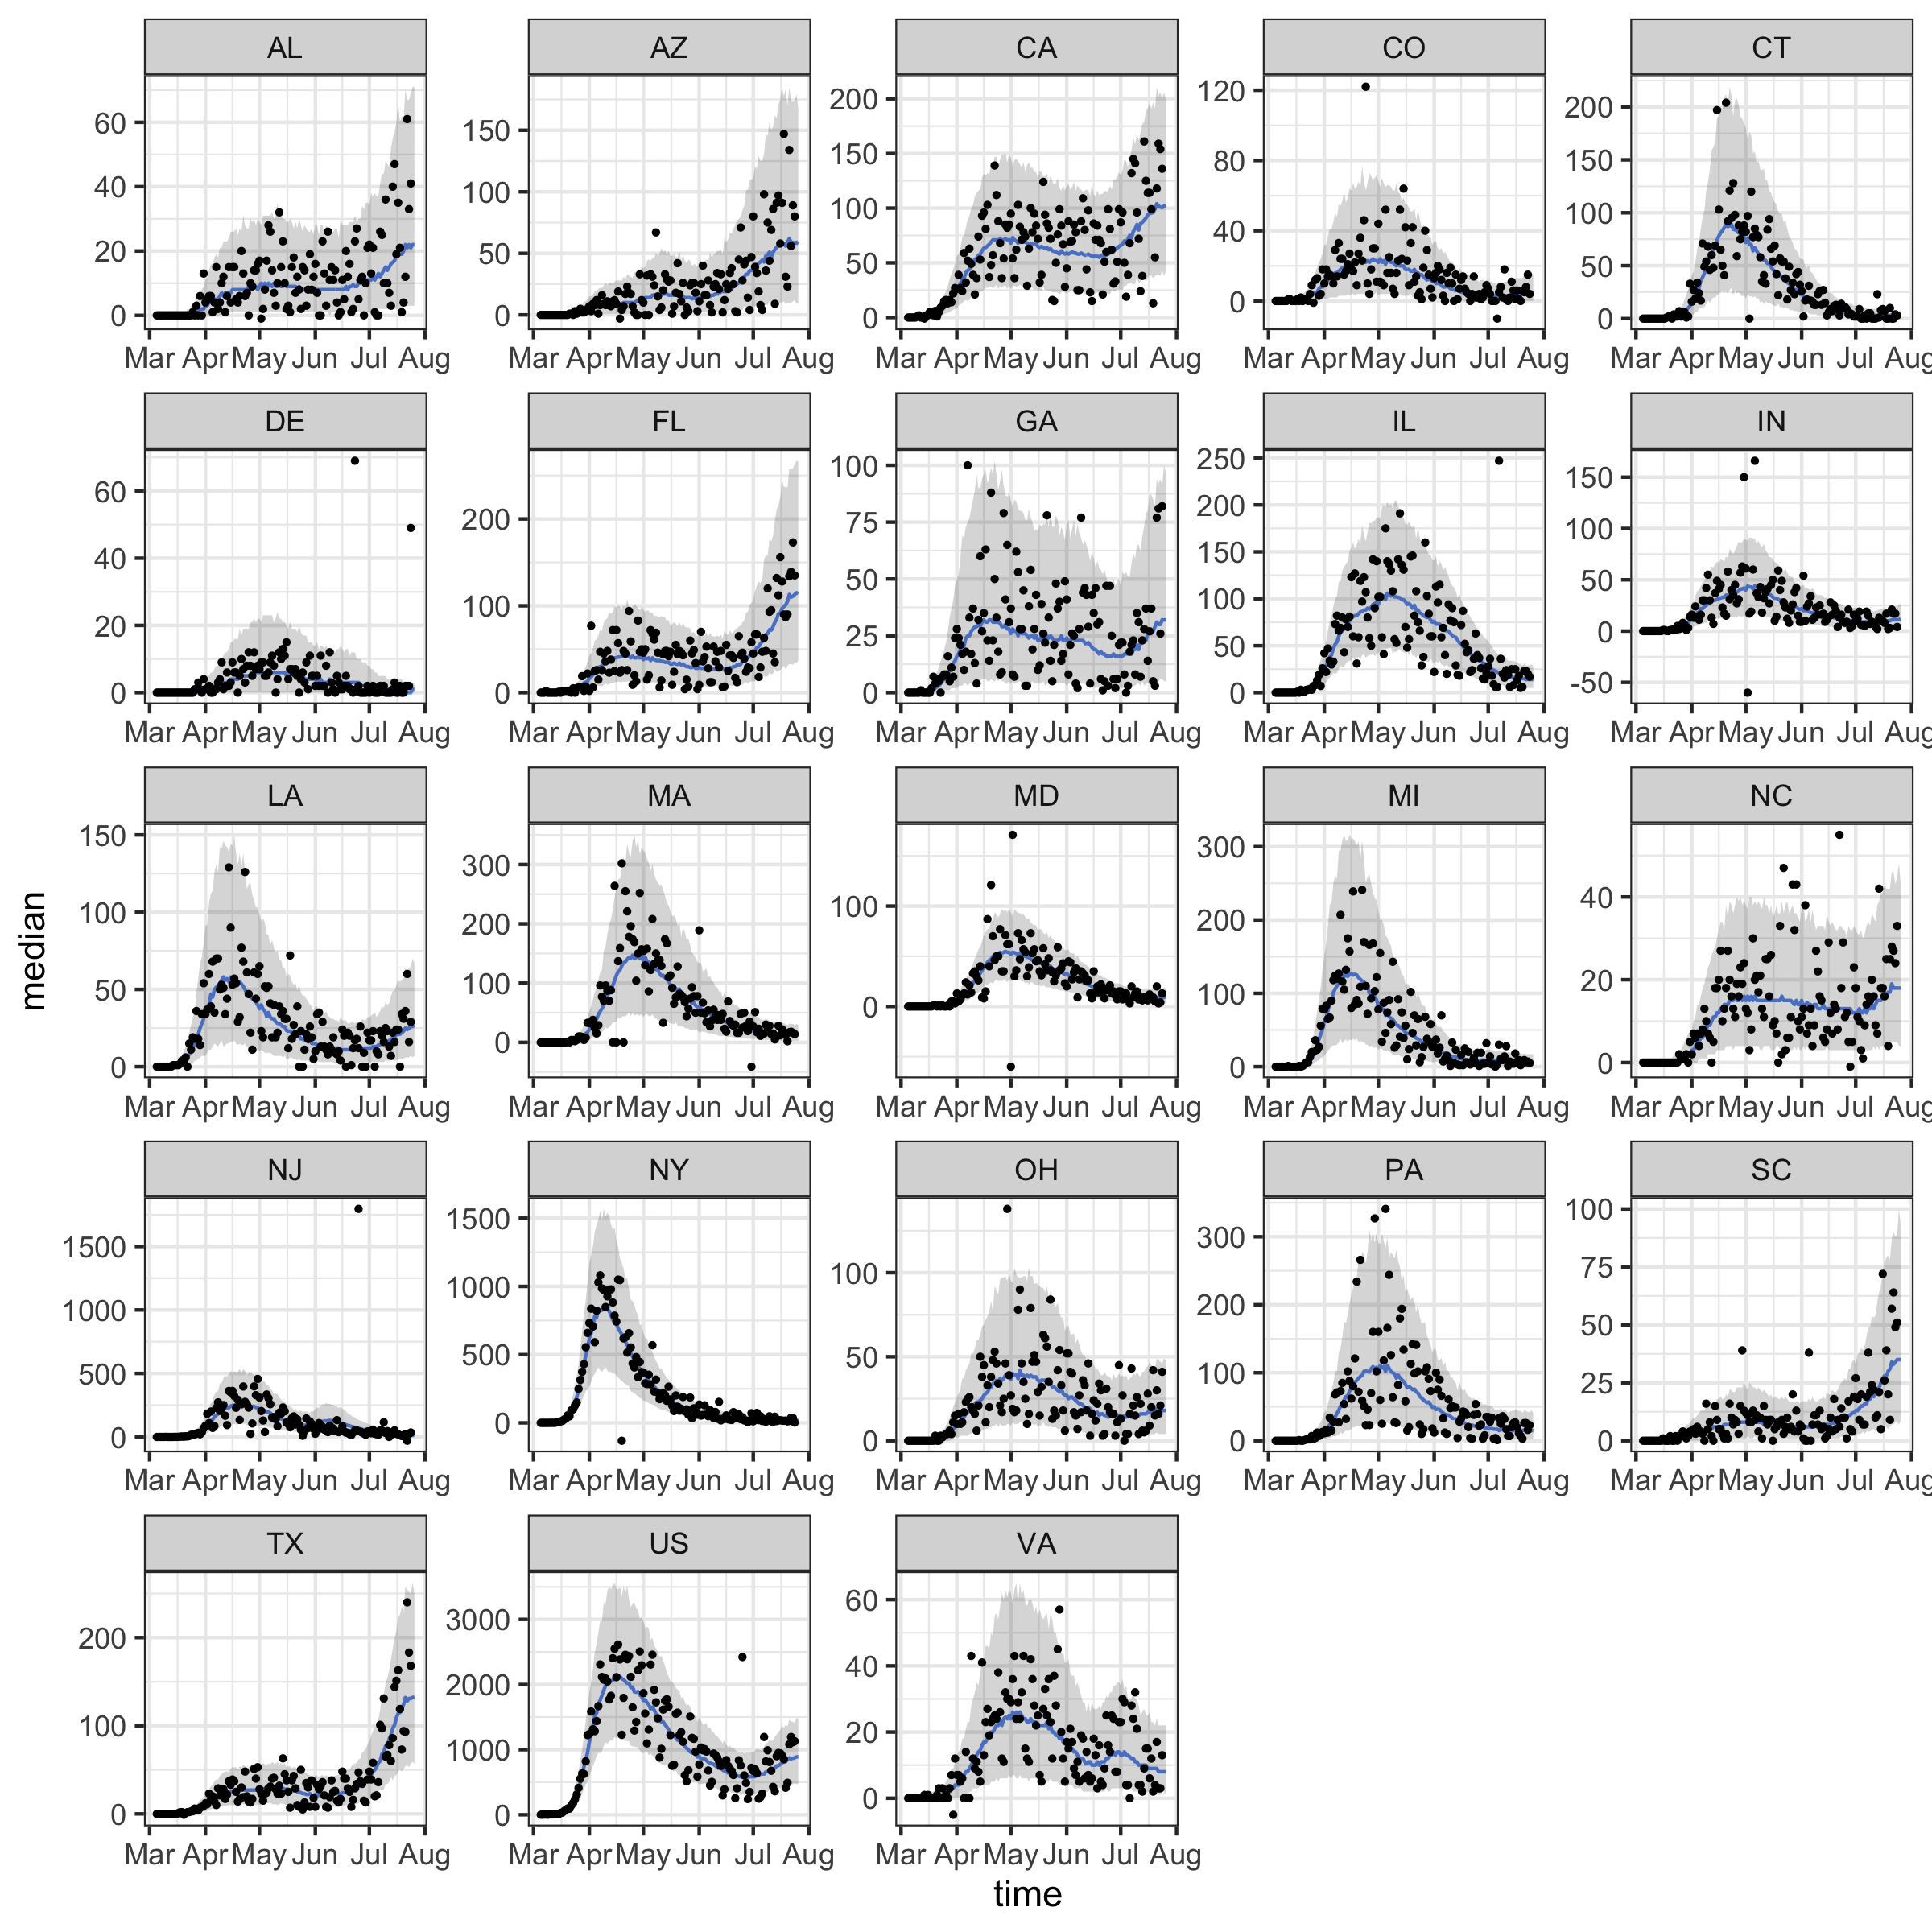
\includegraphics[scale=.2]{fit_and_forecast_results.png}

\caption{Example fit and forecast for states with over 50 incident deaths.}
\label{fig:fit_and_forecast_results}
\end{figure}

	
 
\begin{figure}
  \centering
     \begin{subfigure}{.5\textwidth}
  \centering
    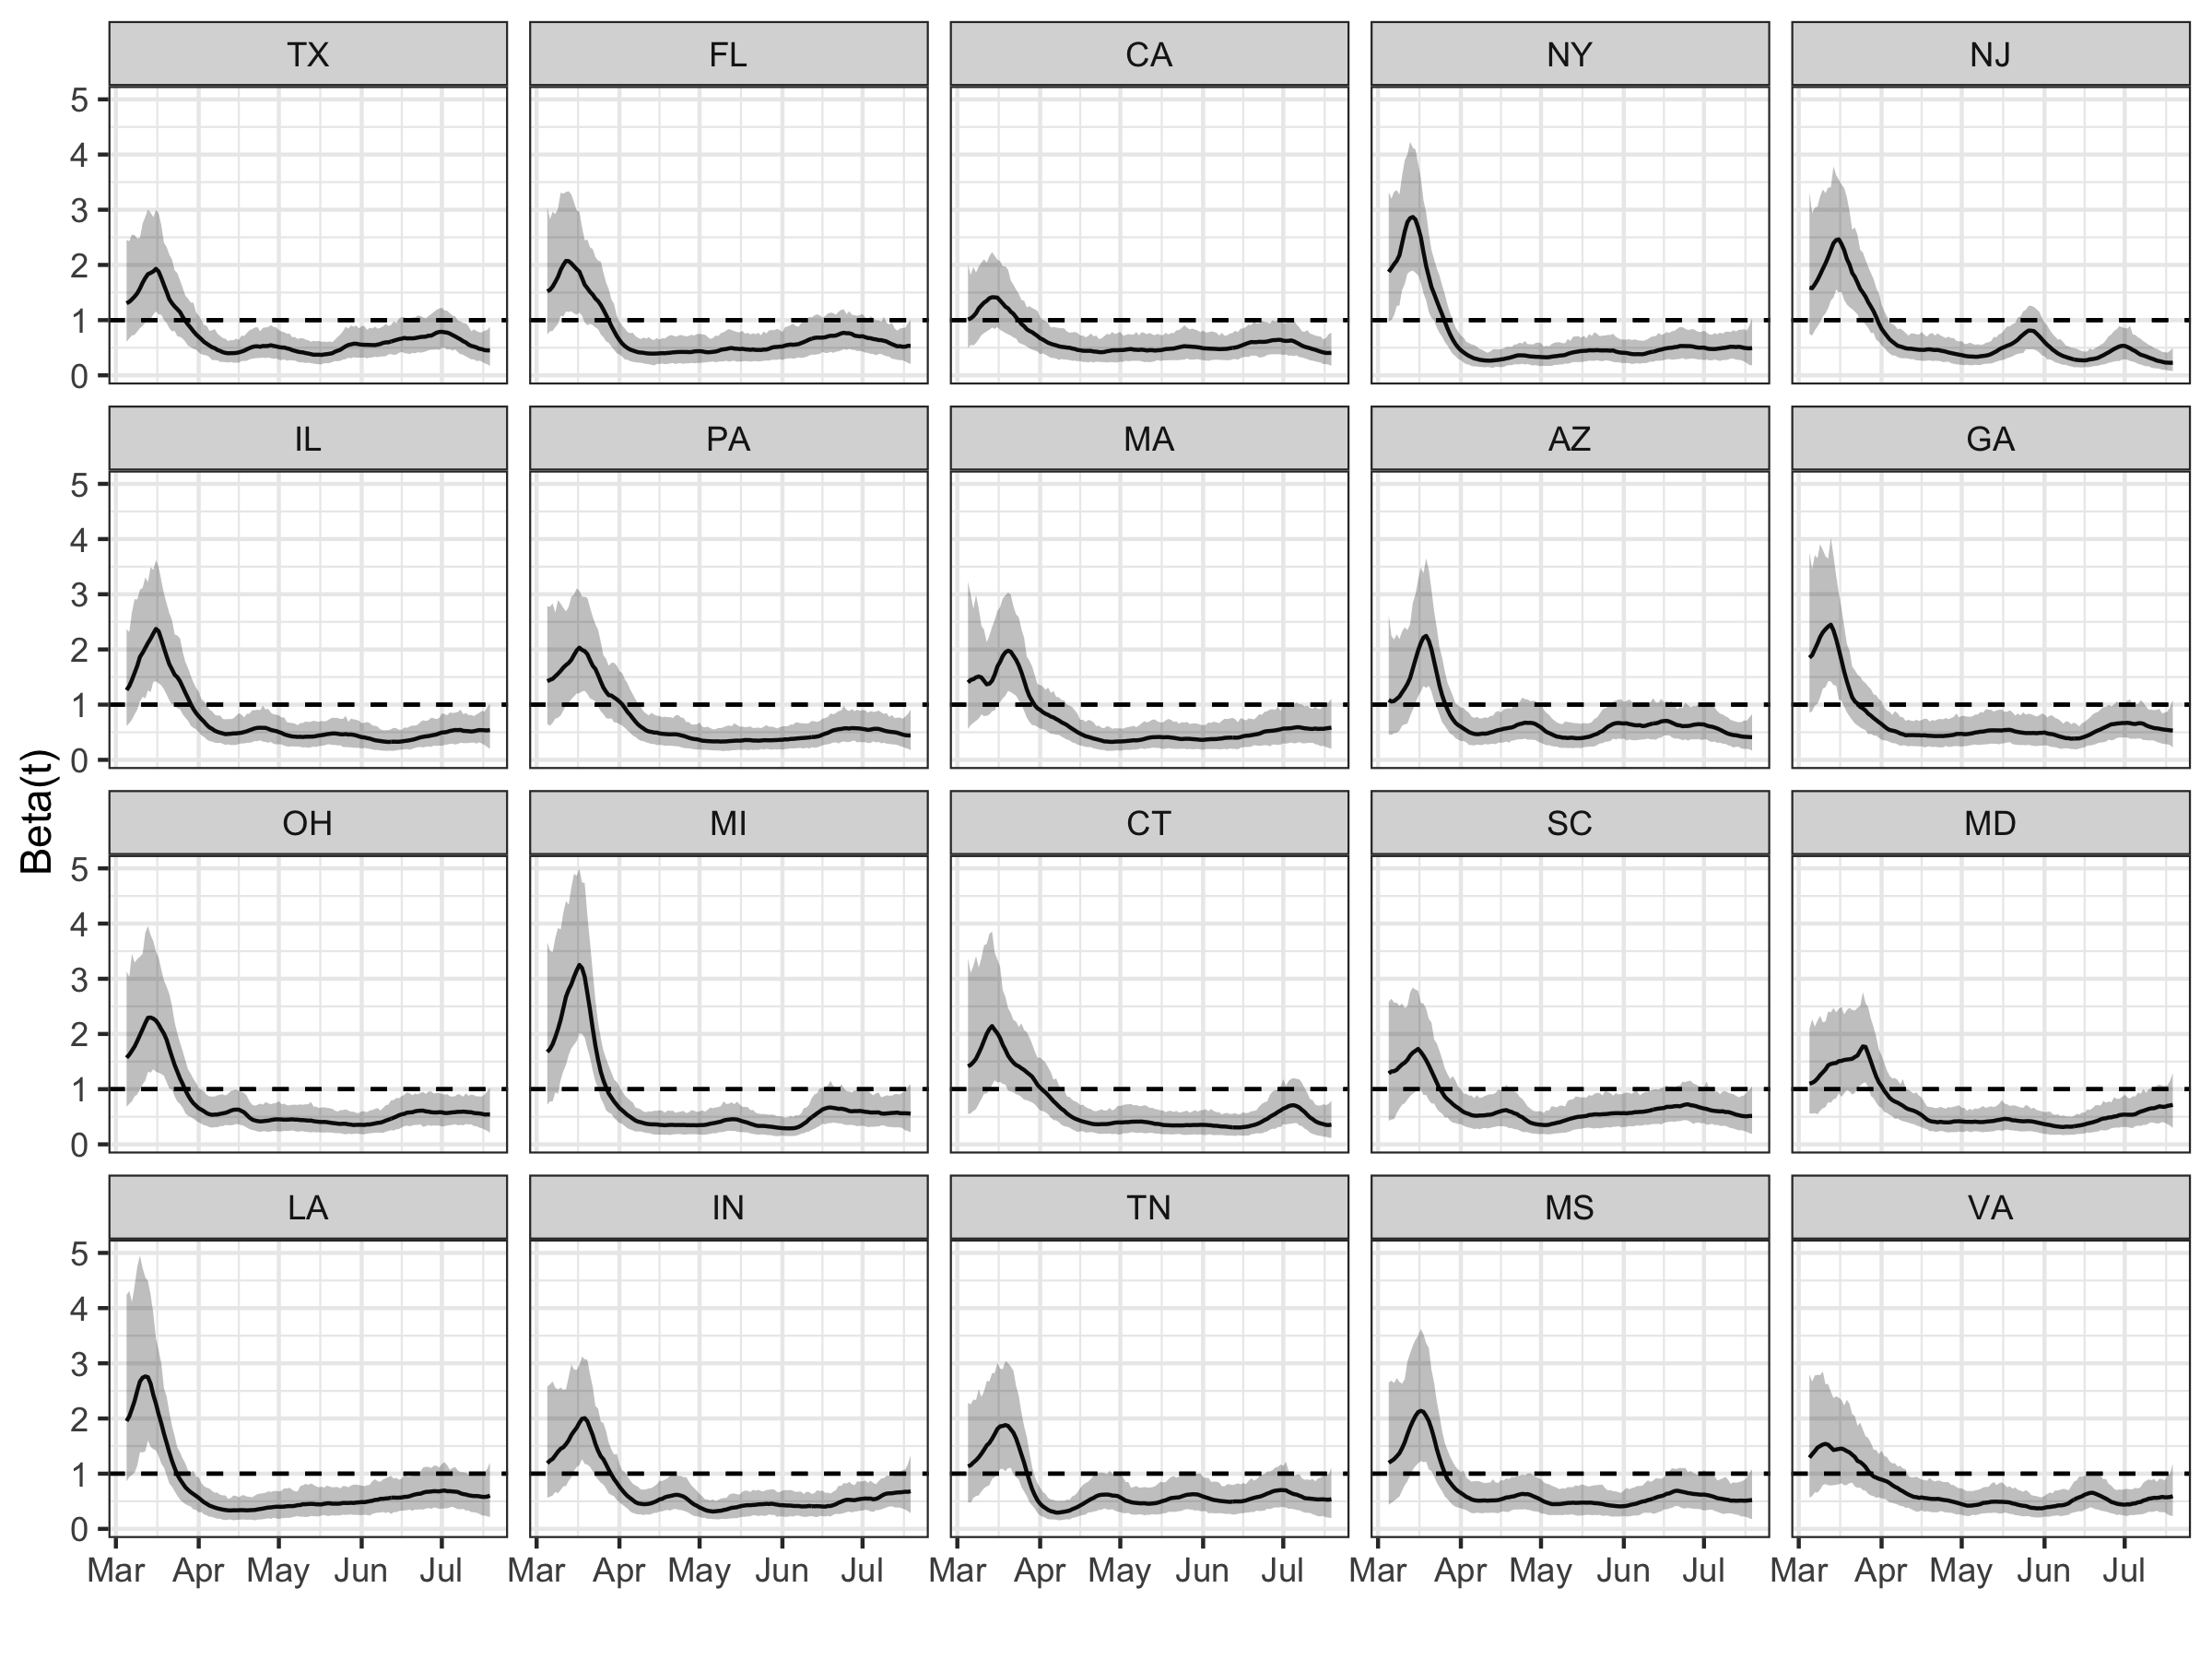
\includegraphics[scale=.1]{beta_t_plot.png}
    \caption{Time varying-beta.}
\end{subfigure}%
\begin{subfigure}{.5\textwidth}
  \centering
    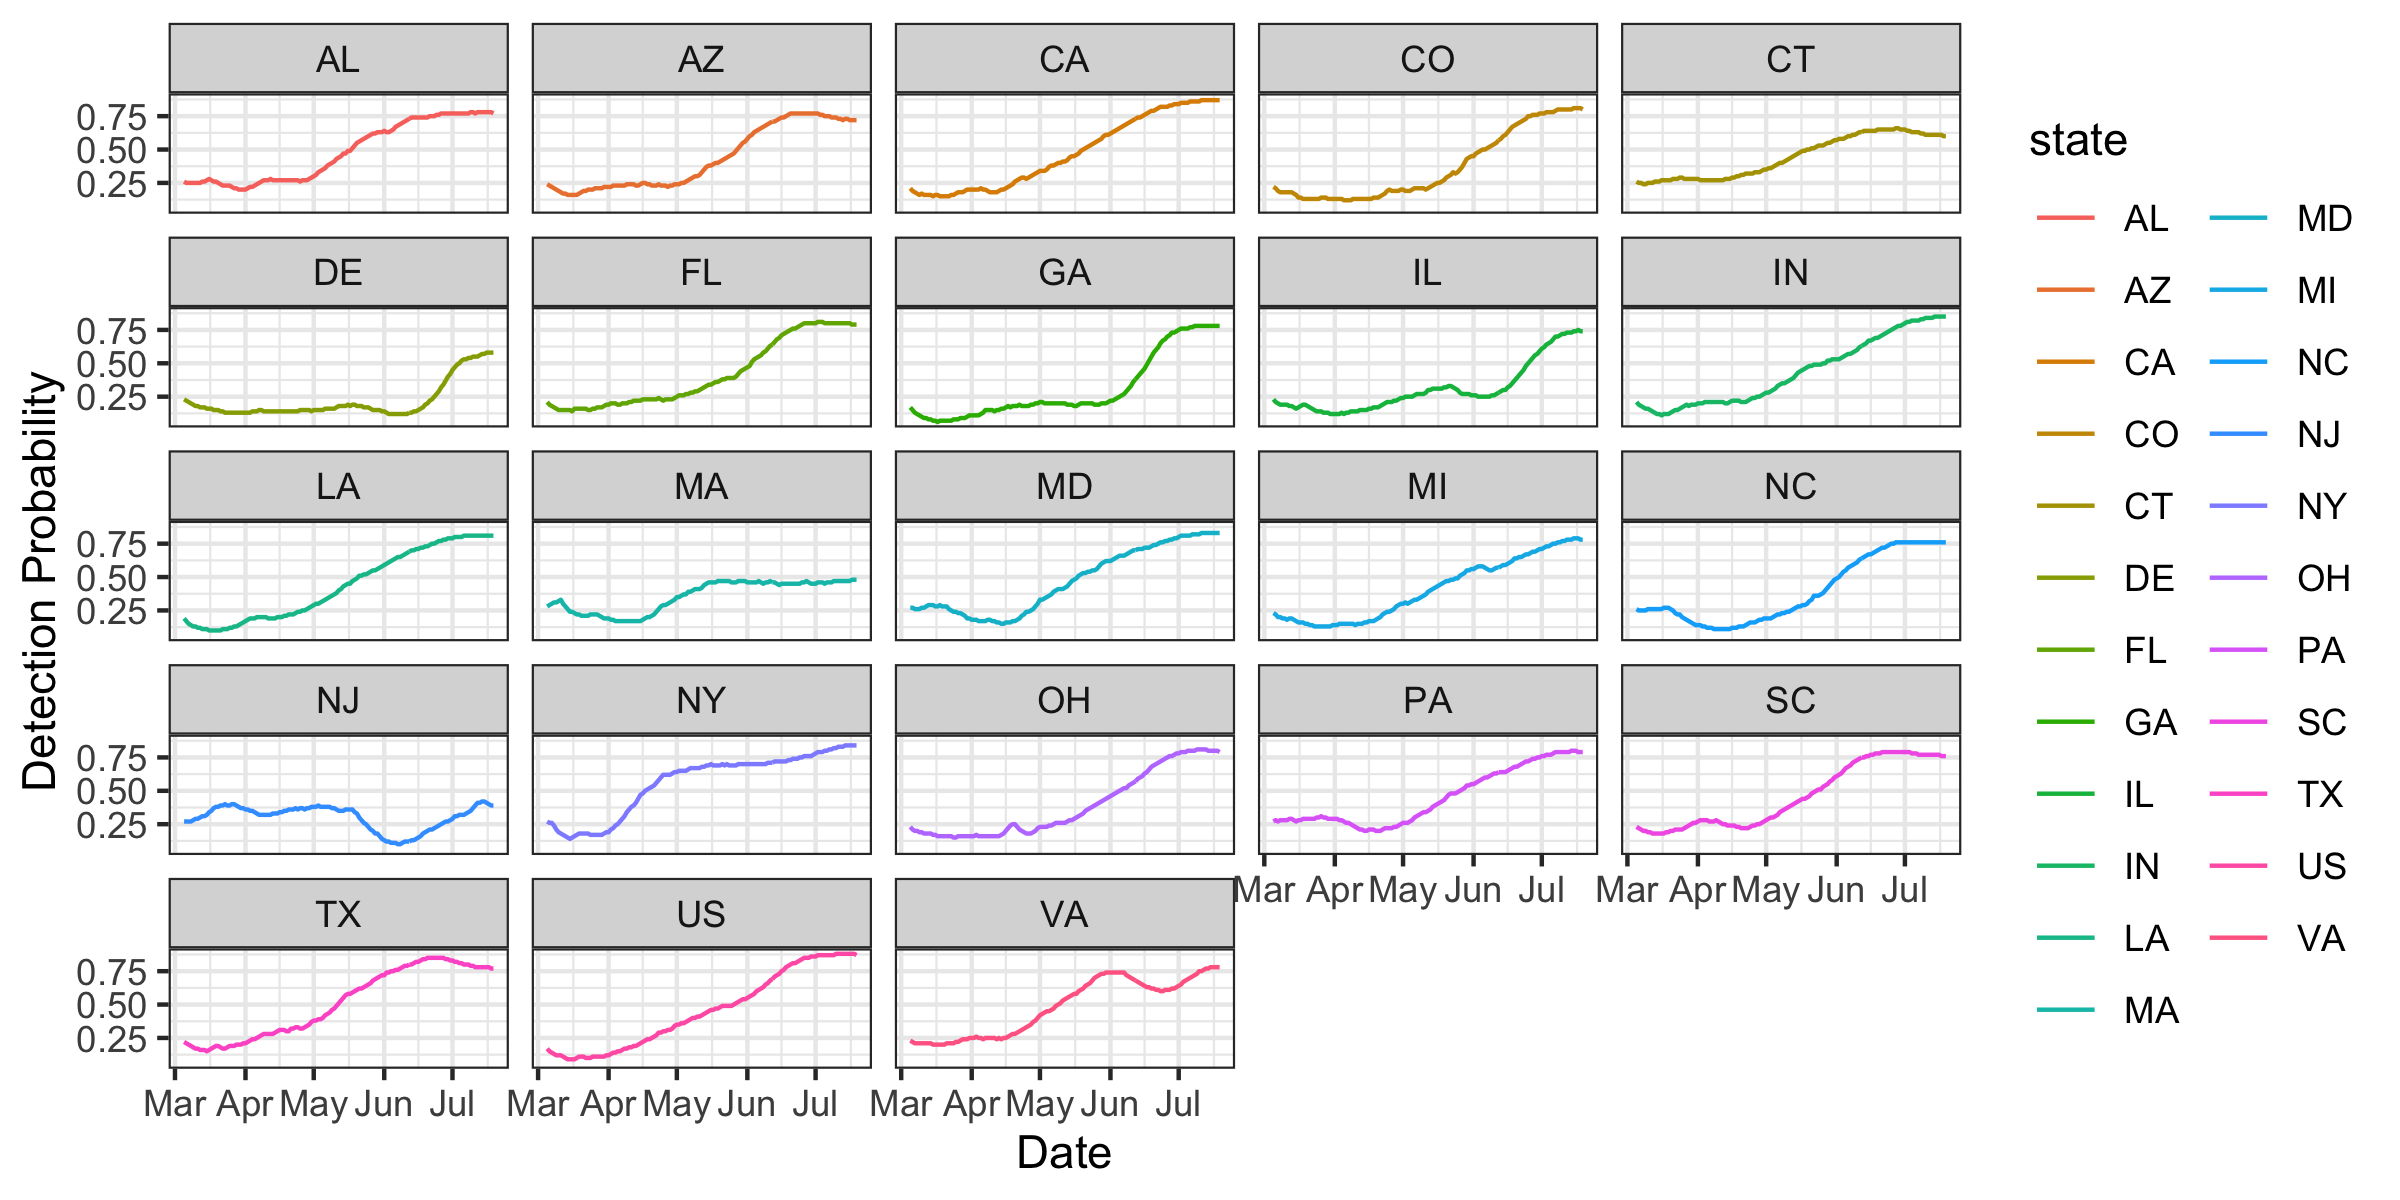
\includegraphics[scale=.1]{detection_plot.png}
    \caption{Time-varying detection probability}
\end{subfigure} 
 \caption{  A) Time varying beta parameter for four example states. We can clearly see that the random walk is able to non-parametrically account for the non-pharamceutical interventions. B) Time varying detection probability for four example states. The time varying detection random walk is able account for the increase in testing. }
\label{fig:model_details}
\end{figure}

\begin{figure}
  \centering
     \begin{subfigure}{.5\textwidth}
  \centering
    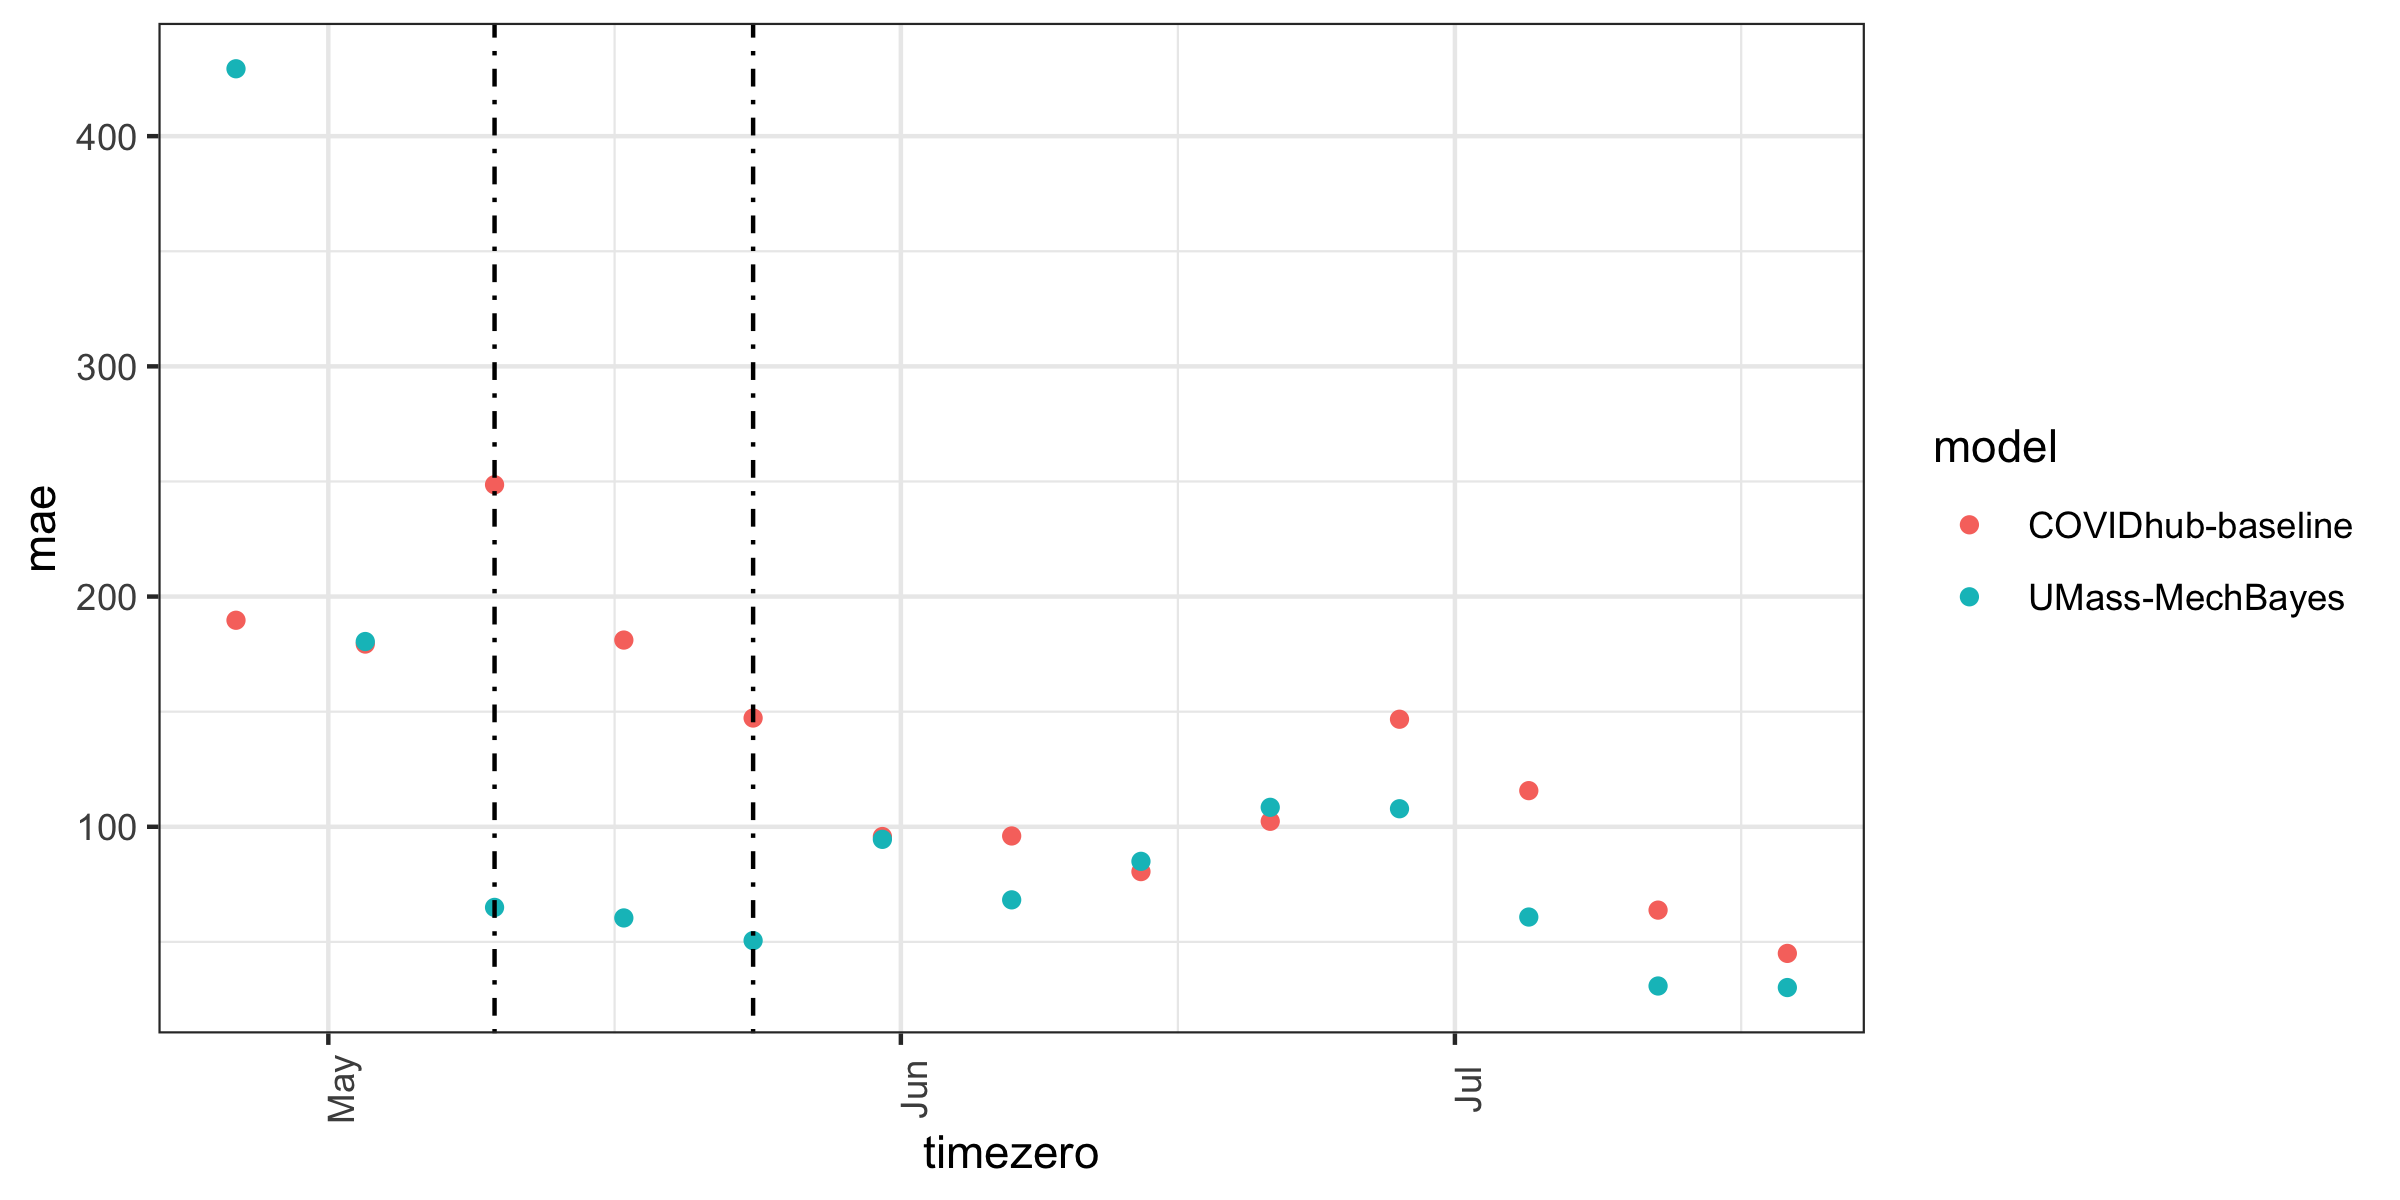
\includegraphics[scale=.1]{mae_results_by_time_zero.png}
    \caption{MAE by timezero}
\end{subfigure}%
\begin{subfigure}{.5\textwidth}
  \centering
    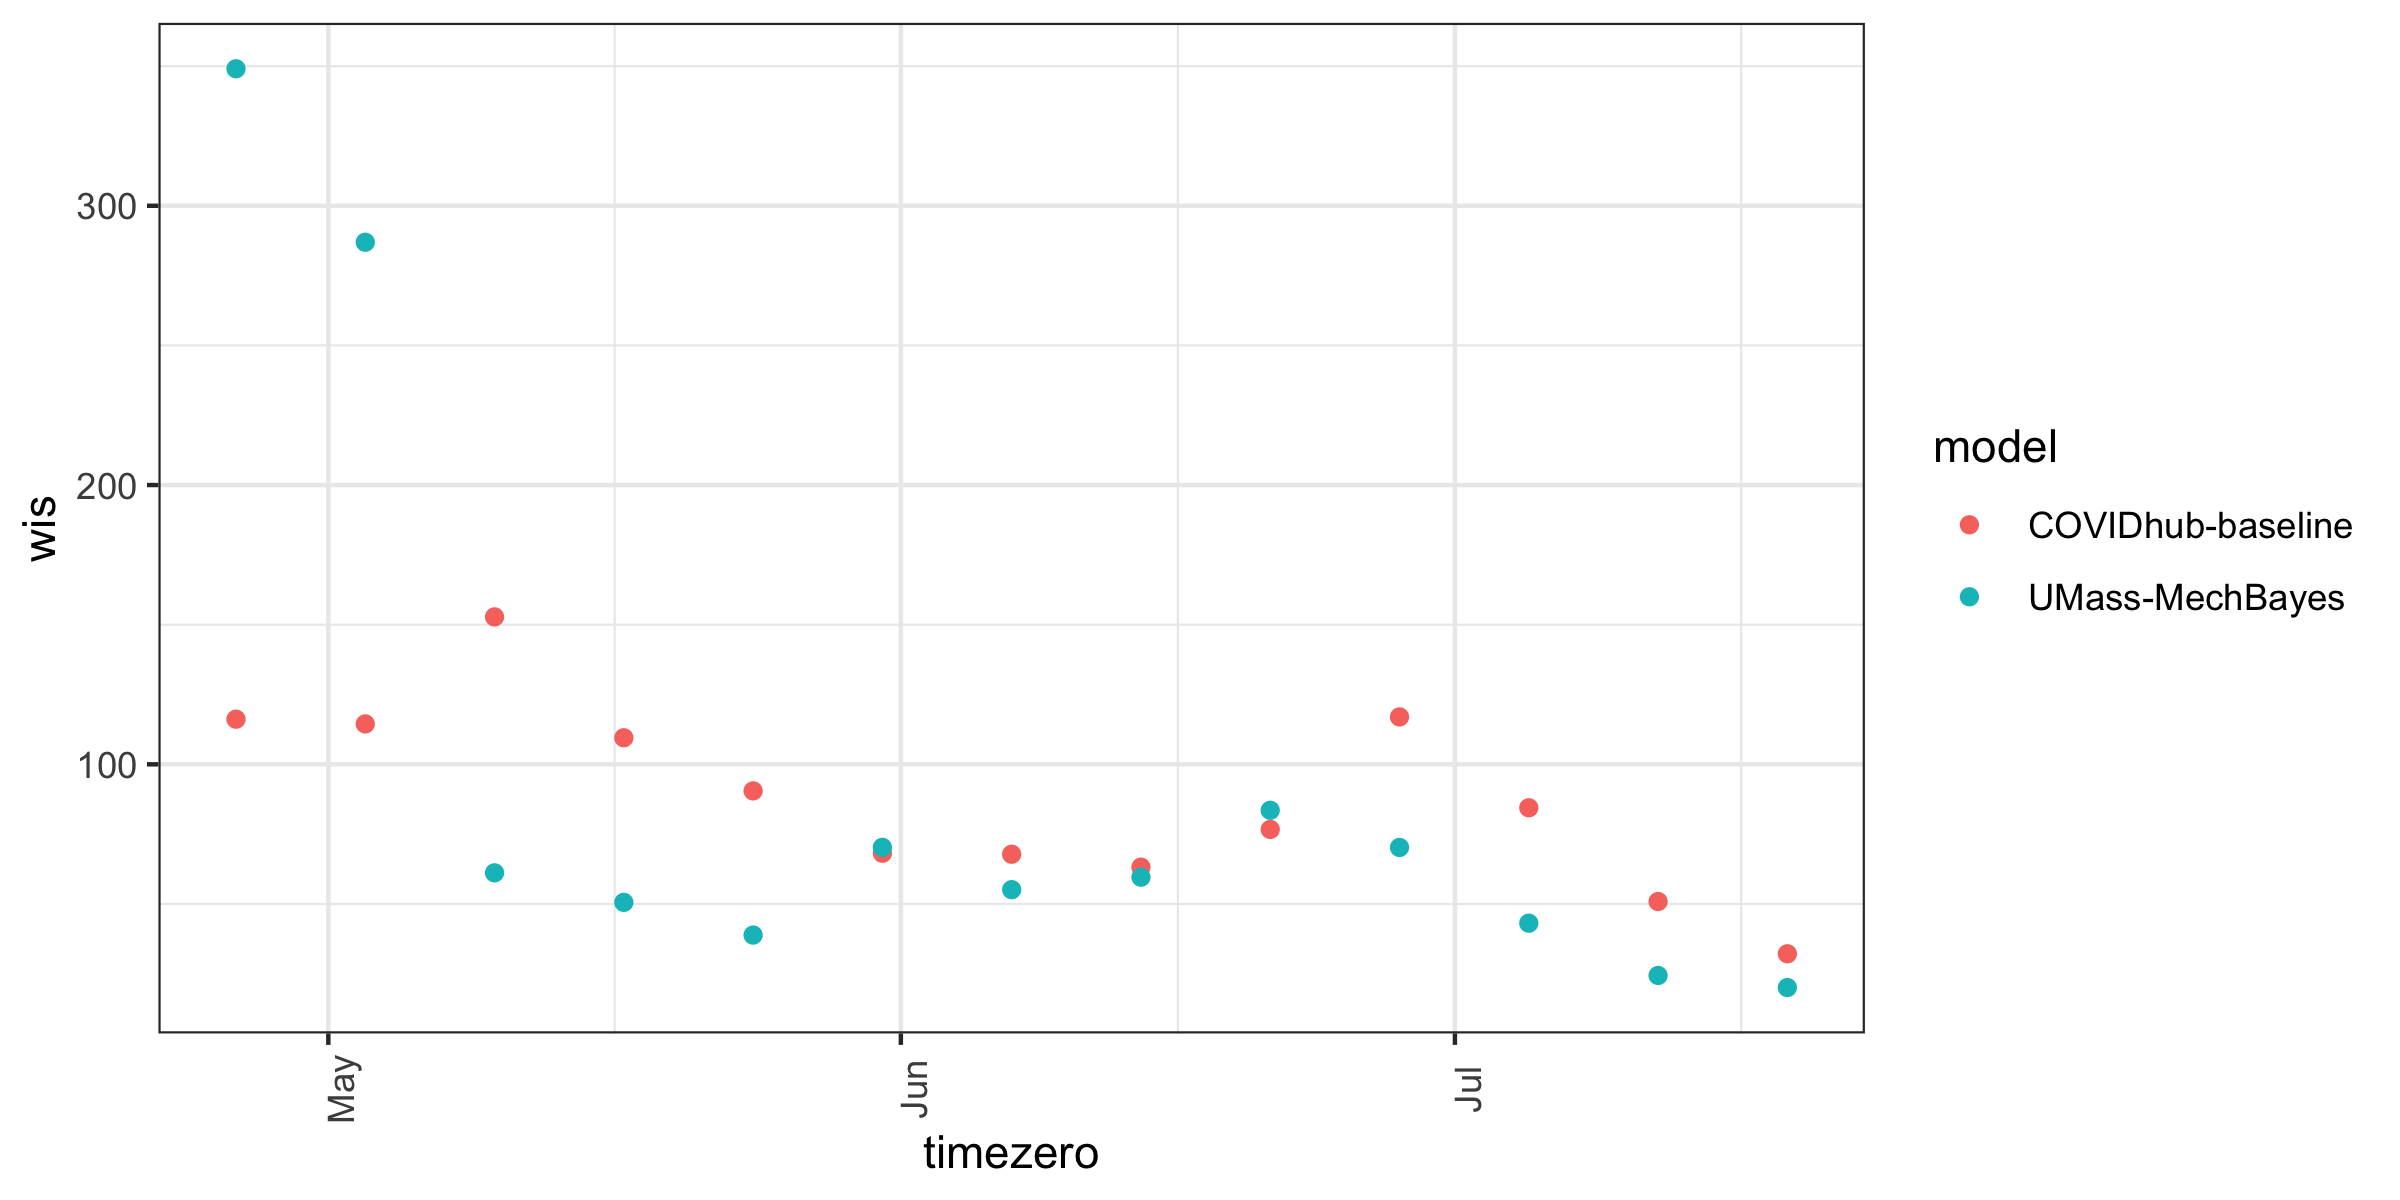
\includegraphics[scale=.1]{wis_results_by_time_zero.png}
    \caption{WIS by timezero}
\end{subfigure}
\begin{subfigure}{.5\textwidth}
  \centering
    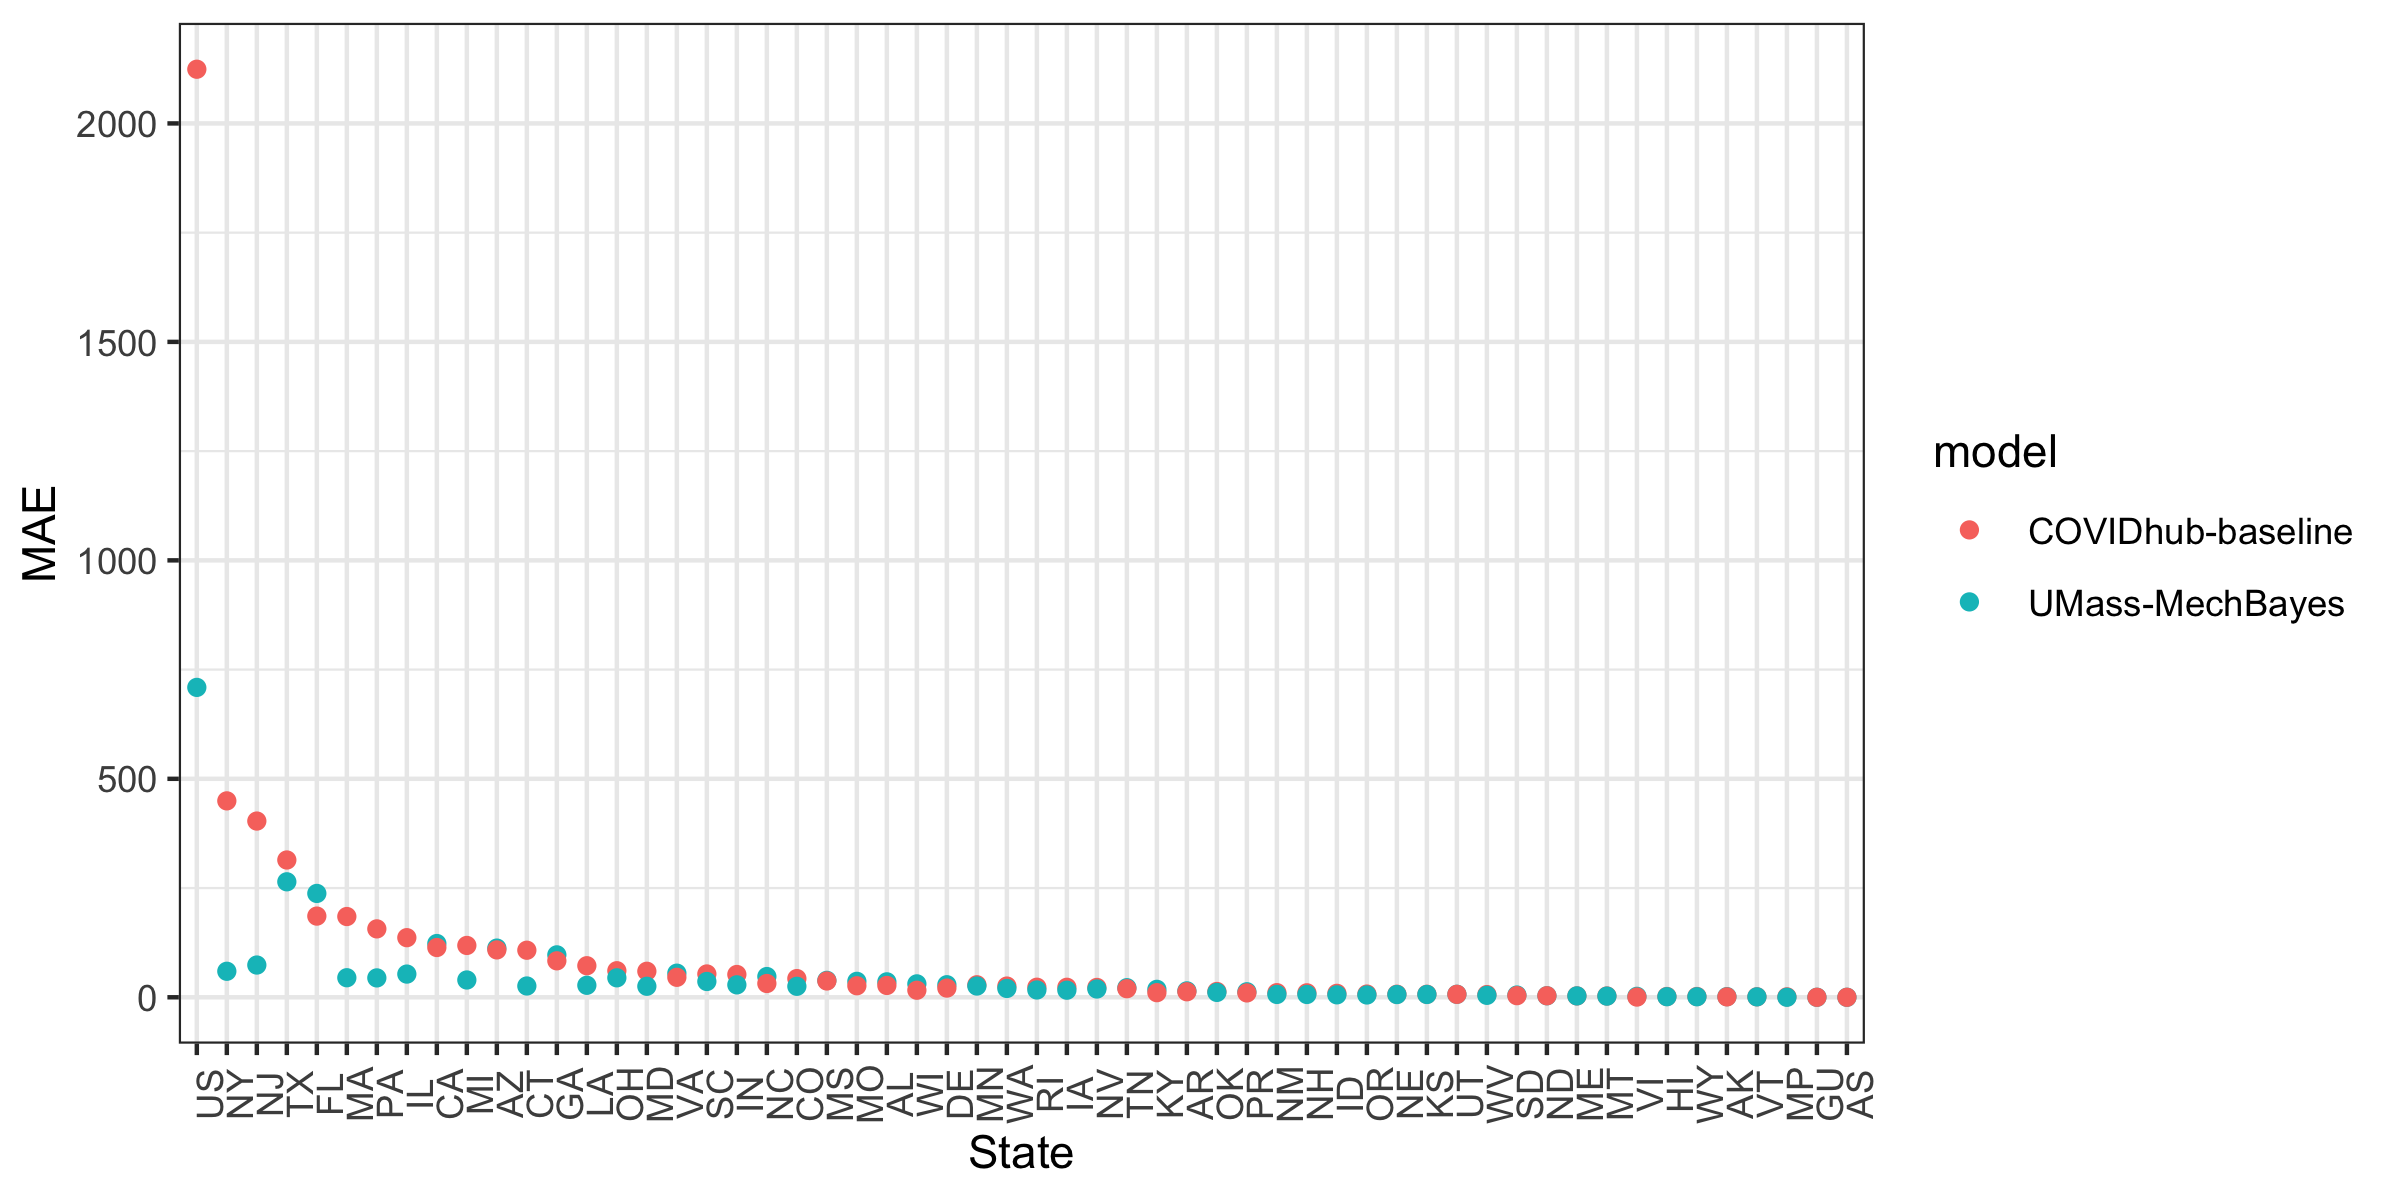
\includegraphics[scale=.1]{mae_results_by_region.png}
    \caption{MAE by region}
\end{subfigure}%
\begin{subfigure}{.5\textwidth}
  \centering
    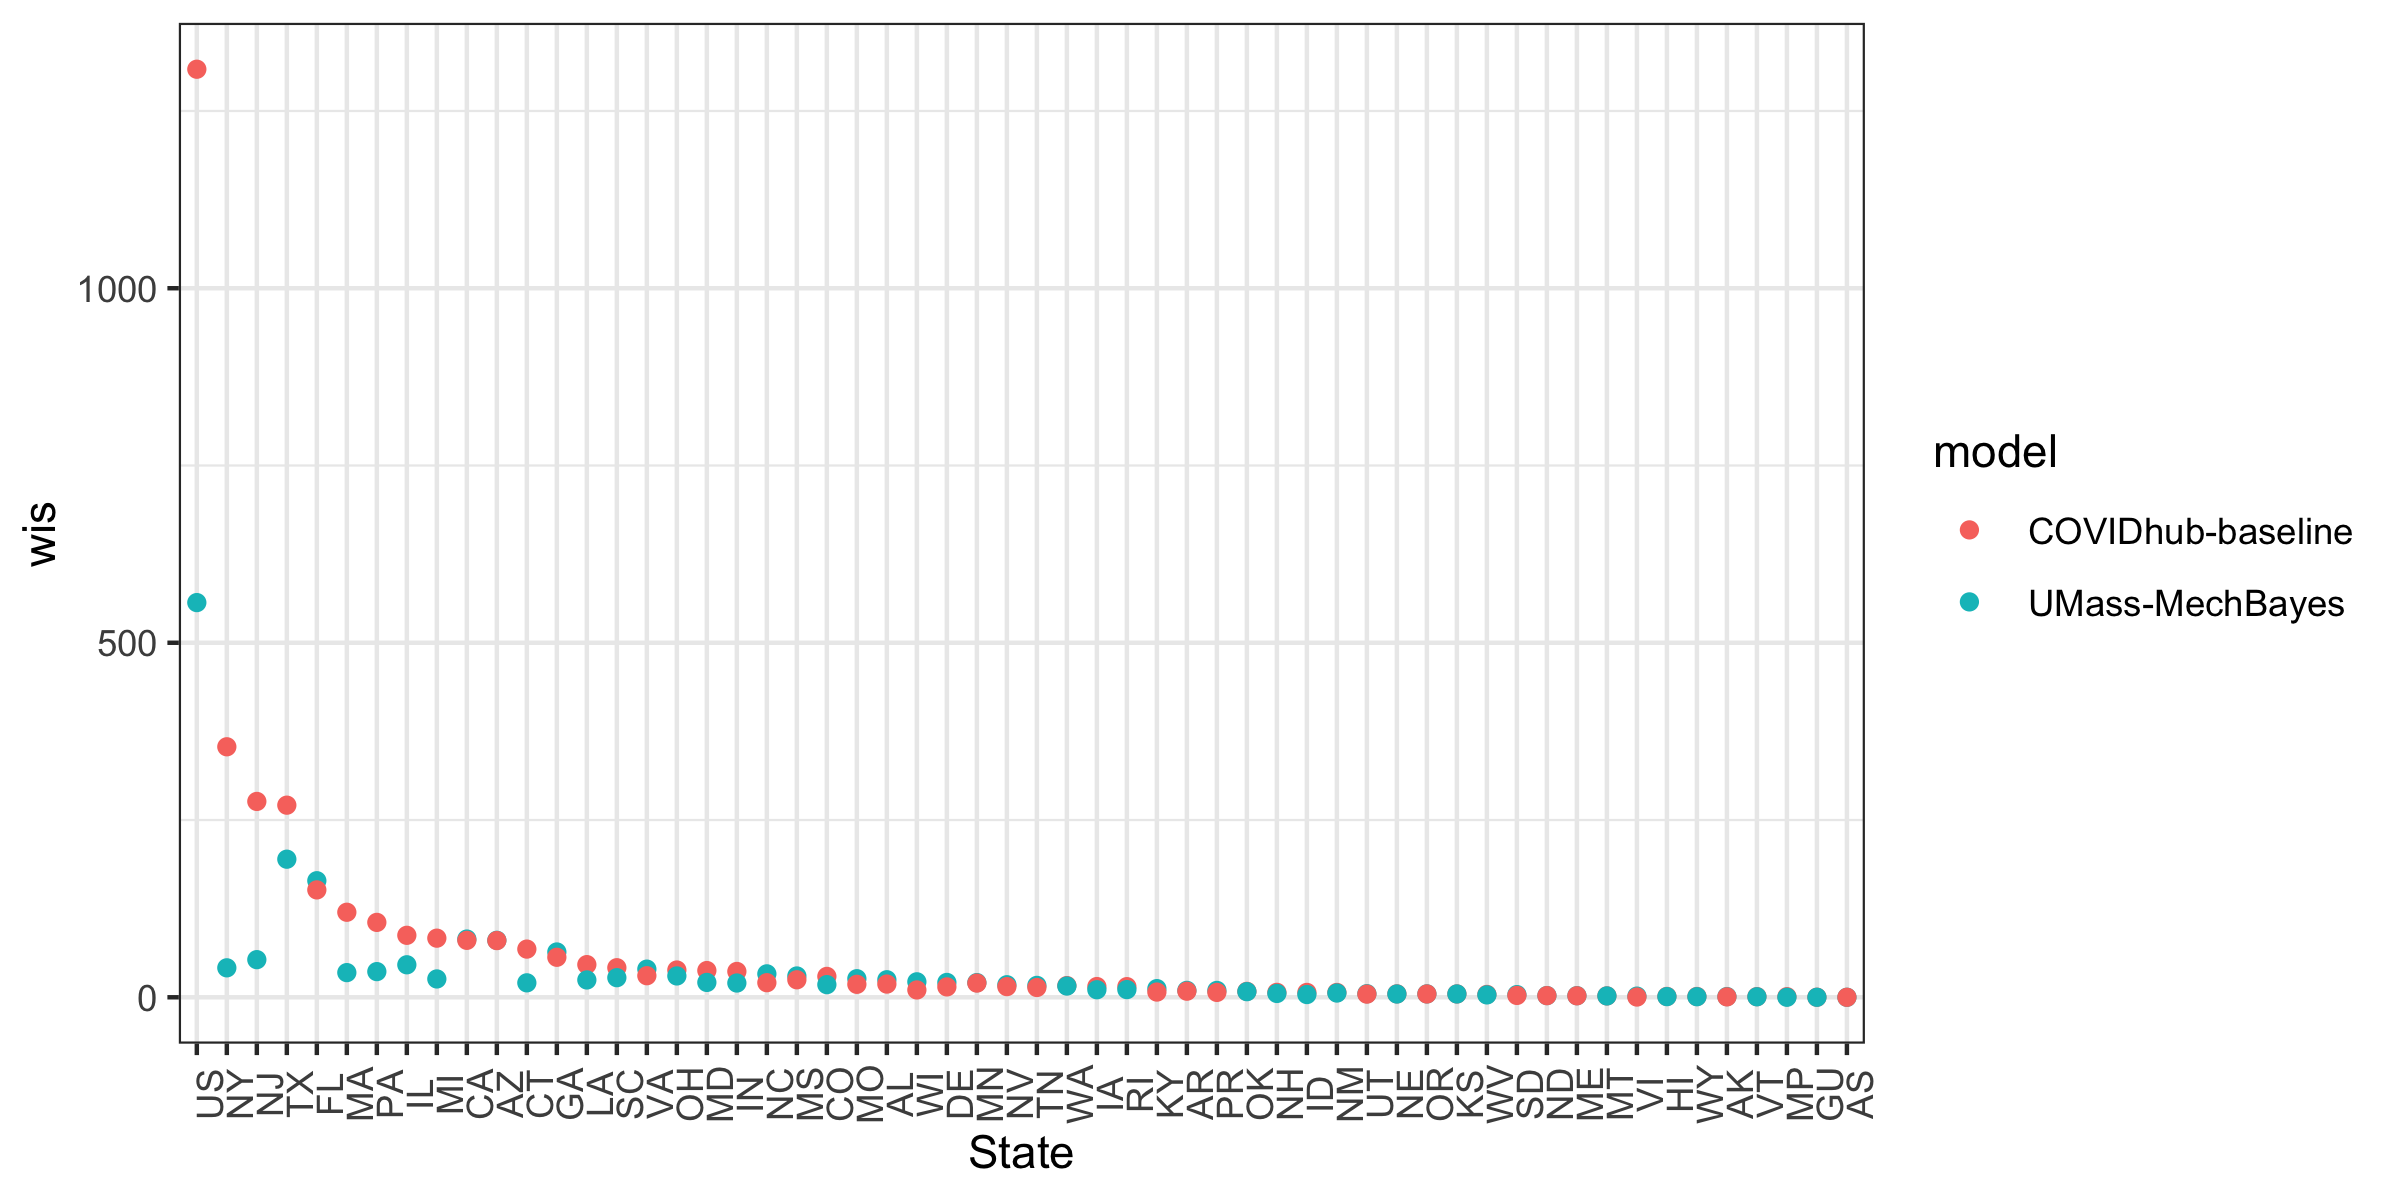
\includegraphics[scale=.1]{wis_results_by_region.png}
    \caption{WIS by region}
\end{subfigure}
\begin{subfigure}{.5\textwidth}
  \centering
    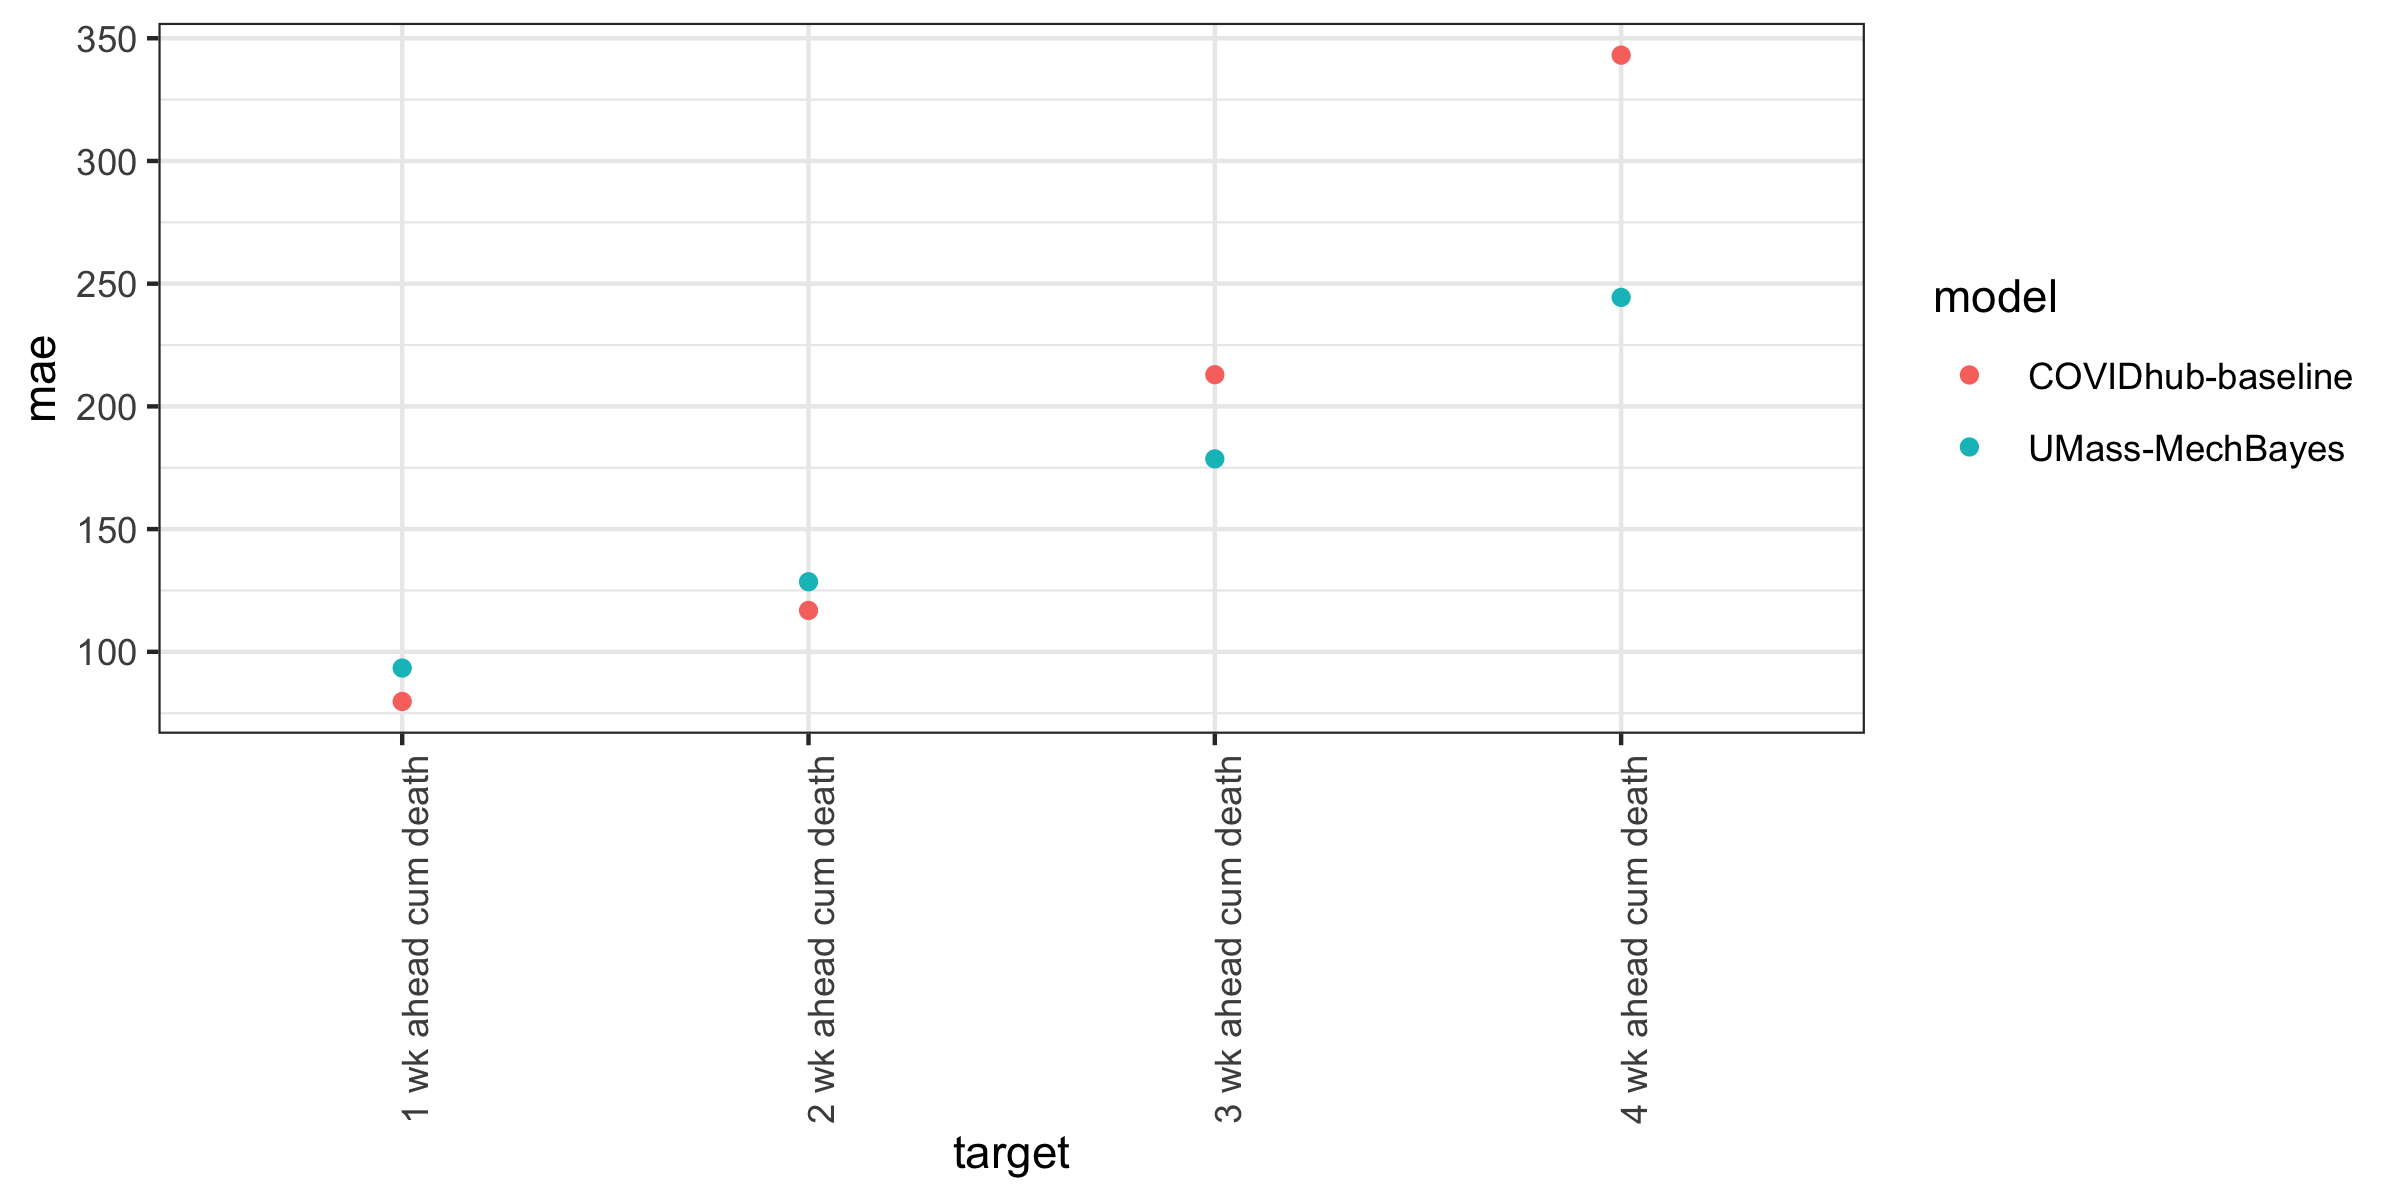
\includegraphics[scale=.1]{mae_results_by_target.png}
    \caption{WIS by target}
\end{subfigure}%
\begin{subfigure}{.5\textwidth}
  \centering
    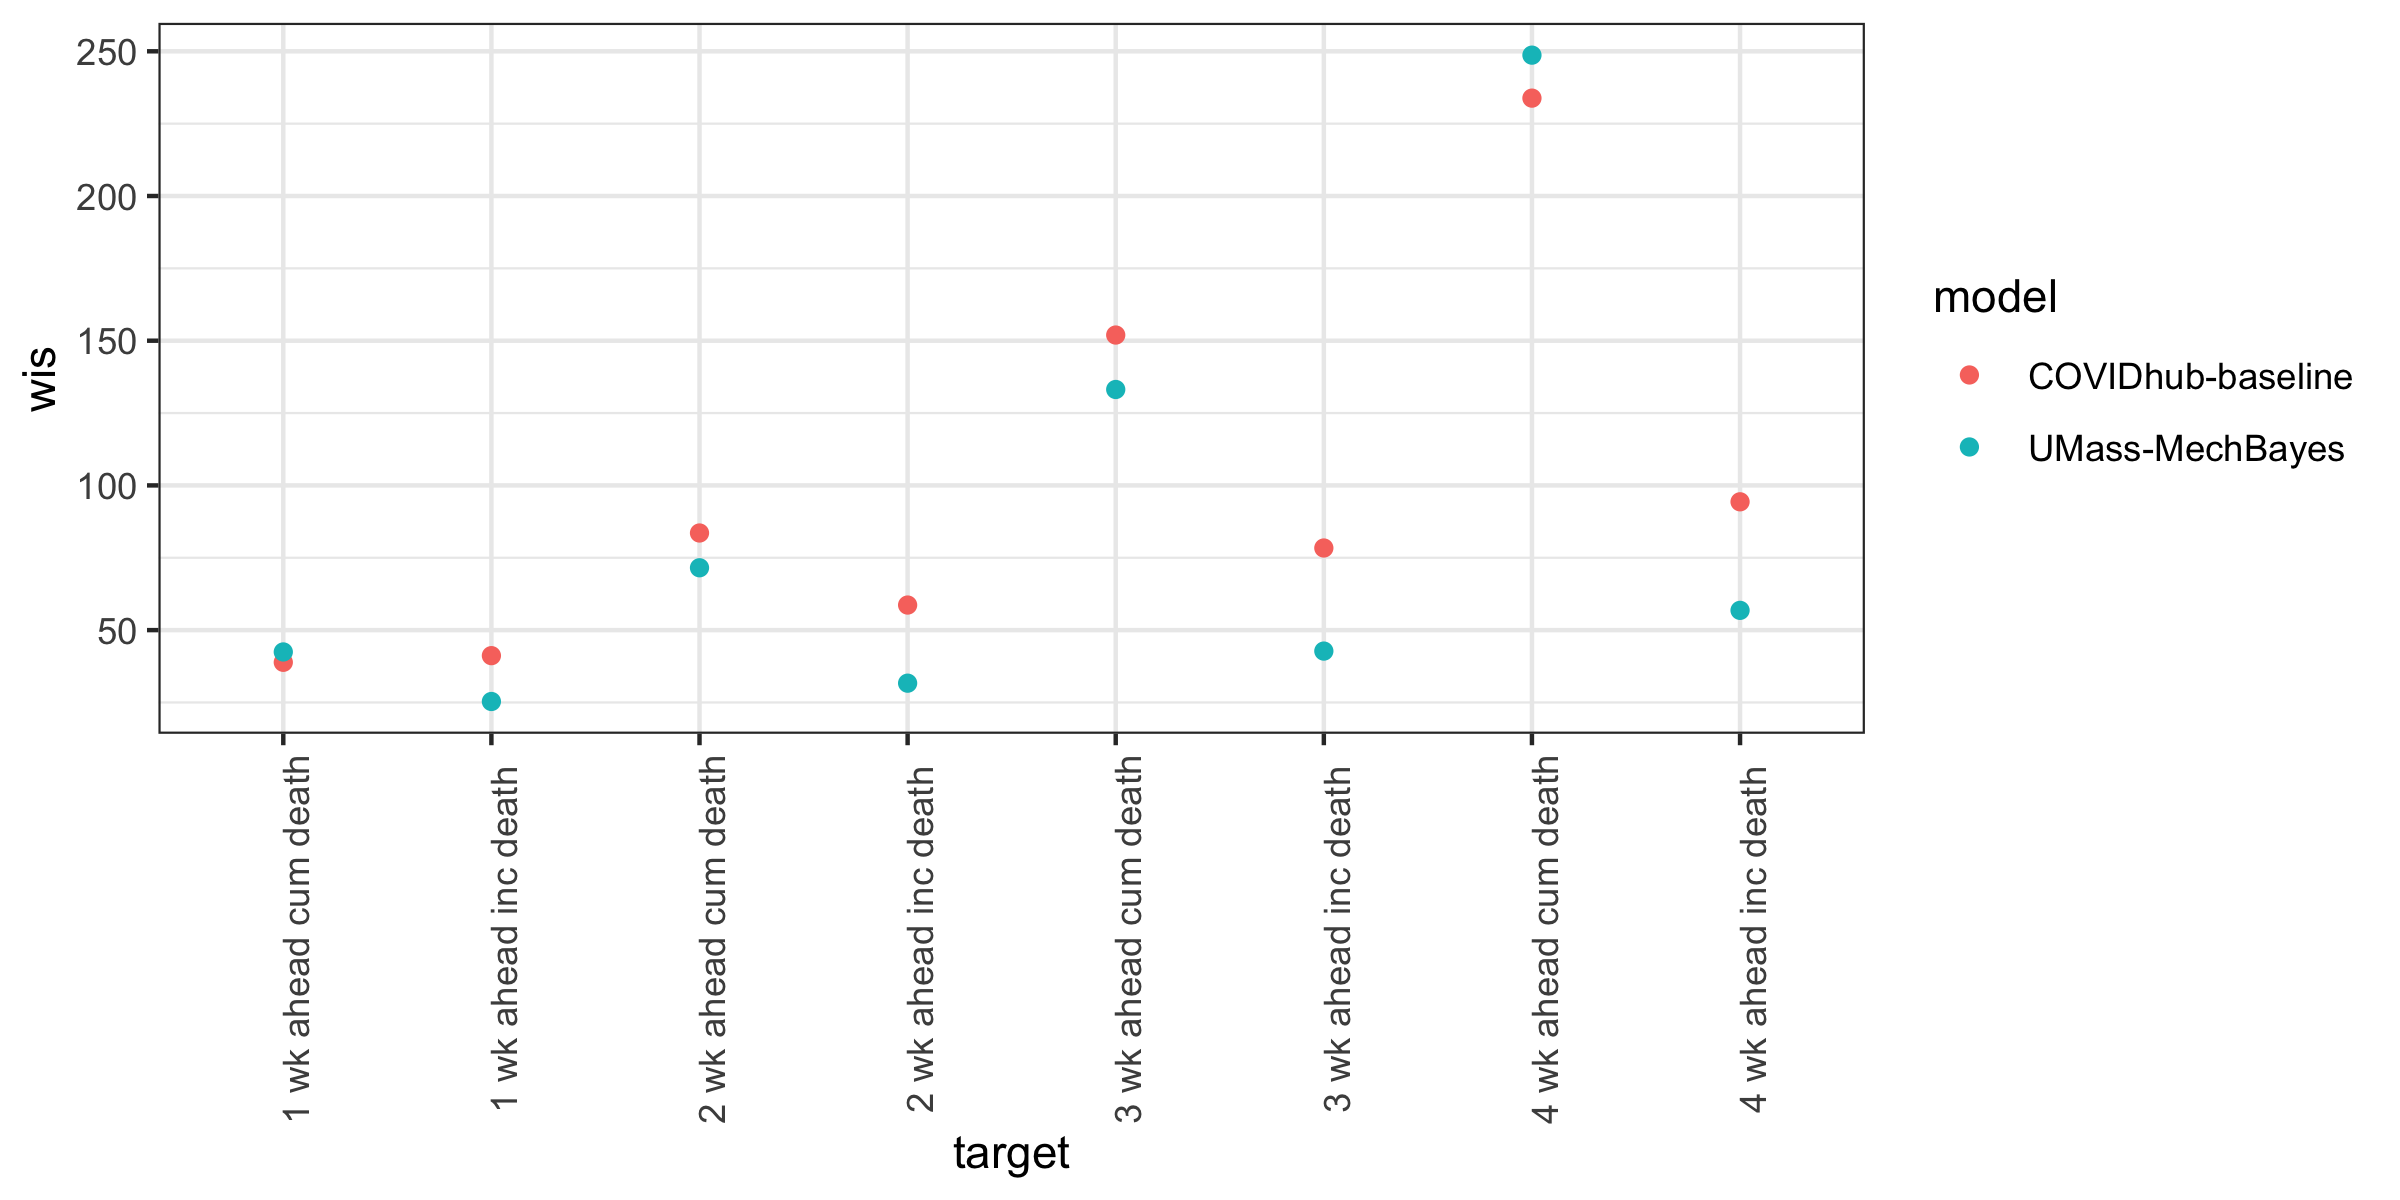
\includegraphics[scale=.1]{wis_results_by_target.png}
    \caption{WIS by target}
\end{subfigure}%

\caption{Scores from COVID-HUB broken down by region, target and timezero. Here we can see that the MechBayes model improves in both MAE and WIS over time, consistently beating the baseline model in the month of July 2020.  }
\label{fig:covidhub}
\end{figure}


We can see from Figure \ref{fig:fit_and_forecast_results} that MechBayes version 3 is able to accurately model the observed data in the three example states (NY,CA,FL) as well as the US. The model is able to adapt to highly variable incident death reporting, variable transmission rates, and overall heterogeneity of incidence curves. The model is also able capture the uncertainty of the differential equation parameters well enough to produce well calibrated prediction intervals. Figure \ref{fig:fit_and_forecast_results}  shows intervals at the 50\%,80\% and 95\% levels. However, we can also see that in some states, such as California and Florida, the model is biased high, with all observations outside of the 95\% prediction interval falling below. Figure \ref{fig:fit_and_forecast_results}  also shows 4 weeks of daily forecasts, along with the daily observed incidence for 1 week out. We can see that the predictions are tracking the data even under the weekly reporting cycles. 

We can see from Figure \ref{fig:model_details} that MechBayes is able to learn to adapt to the evolving pandemic situation. Panel A shows the time-varying transmission $\beta(t)$ for three example states, CA, FL, and NY as well as the U.S. We can see that $\beta(0)$ is centered on our prior but as data comes in, the estimate increases. This is especially true in NY, where the epidemic took off quickly in March. However, the model is then able to adjust to the varying levels of non-pharamceutical interventions present in each of the three states as well as across the U.S. This radically reduces the transmissibility parameter by the first week of April 2020. This is consistent with a peak in overall deaths two weeks later in mid-April 2020. There seems to be some estimation issues at the boundary of $\beta(t)$ where the number of cases does not match the number of deaths, since the cases have not yet converted to deaths. This results in the model underestimating transmissibility to reduce the flow through the compartments. \textbf{Need to think on this a bit}

We can also see from Figure \ref{fig:model_details}  that MechBayes is able to account for the drastic increase in testing that has occurred across the U.S. since March 2020. Panel B also shows that our prior estimate of 30\% of cases being detected, may have been too high, as all regions show a dip in detection probability before climbing again. Note that interpreting this strictly as time-varying detection is obscuring the fact that this parameter $p_{t,d}$ can soak-up any excess variation beyond the ability of cases and the case-fatility ratio to explain the number of deaths. That is, the time-varying detection probability is able to "de-couple" cases and deaths beyond the case-fataility ratio regardless of the underlying reason (whether that be an increase in testing or shifting age distribution of cases). Thus, interpretation of this parameter as a strict mapping to testing is incorrect. As a forecasting model, we only need the ability to non-parametrically model deviations and reporting issues in cases.

We next turn to the comparison of MechBayes against the COVID-HUB baseline model. This baseline model uses the previous daily incident as the mean forecast for the current daily incidence, along with  bootstrapped prediction intervals from historical changes in daily incidence. See COVID-HUB for more details. \cite{COVID-HUB}. 

We begin by breaking down the results by week the forecast was made (timezero) and averaging over both region and target. As we can see from Figure \ref{fig:covidhub} (A,B), MechBayes V1 did not outperform the COVID-HUB baseline on MAE or WIS when broken down by timezero. However, MechBayes V2 (the introduction of the time-varying detection probability), outperformed the COVID-HUB baseline model on both MAE and WIS when broken down by timezero. The same is true for MechBayes V3 with the exception of June 26th, where the COVID-HUB baseline model slightly outperformed MechBayes V3. However, as seen in Figure \ref{fig:data}, overall incident deaths were at their lowest across the U.S. in late June and remarkably stable, meaning this week was the hardest of the weeks to beat the baseline model. 

We also break down the results by geographical region, as seen in Figure \ref{fig:covidhub} (C,D). Note that this break-down is averaged over target, but also timezero, meaning that we average over each of the model versions. We feel this is important, as it reflects the real-time accuracy of our evolving model efforts, instead of \textbf{cherry-picking} the best model. However, we still consistent improvements in MAE under MechBayes when broken down by region, with the exception of New York. This is mainly due to MechBayes V1 large MAE for New York in March, where most of the cases (and therefore contribution to MAE) occurred. The WIS results are similar. 

Finally, we break down the results by target by averaging over region and timezero  \ref{fig:covidhub} (E,F) Here we can see uniform improvement over the baseline model by MechBayes in terms of MAE and WIS. We can also see that the MAE increase as horizon increase, which is to be expected. We can also see that incident MAE is lower than cumulative MAE, which is again to be expected due to the lower absolute numbers of incident deaths. Finally, we see the model is slightly better calibrated on incident deaths than cumulative.
%
%\begin{itemize}
%\item MechBayes is almost always better than baseline model when broken down by region, target, and timezero after June 1st 2020.
%\item MechBayes has improved over time.
%\begin{itemize}
%\item First two submissions did not have detection probability random walk
%\item Observations were Normally distributed on cumulative deaths
%\item Switched to current model
%\end{itemize}
%\item Naive baseline is hard to beat
%\item MechBayes is biased high. This comes from uncertainty in the random walk leading to potentially huge growth rates. 
%\end{itemize}   
%   
   
   
   \section{Ablation Results}

We can see from \ref{fig:ablation} that MechBayes Full is consistently better than MechBayes Death Only or MechBayes Fixed Case Detection Probability. The only exception seems to be June 22nd 2020 for the two week ahead target. Late June 2020 is when many states in the U.S. began to see an uptick in cases again, with Texas, Florida, and California seeing their largest total case counts since the beginning of the pandemic. Since MechBayes is conditional on the current level of interventions, forecasts made from June 22nd assumed the same level of intervention present on June 22nd. During this time, each state was re-opening various establishments, while cases were rising. MechBayes Full forecasted an exponential growth in cases, which was reflected in a large over prediction two weeks later on July 4th. 

We can also see that the MechBayes Death Only is consistently better than MechBayes Fixed Case Detection Probability.  This may be evidence that naively including case data, without adjusting for time-varying testing rates, may be worse than not including it at all. 

\begin{figure}
  \centering
     \begin{subfigure}{.5\textwidth}
  \centering
    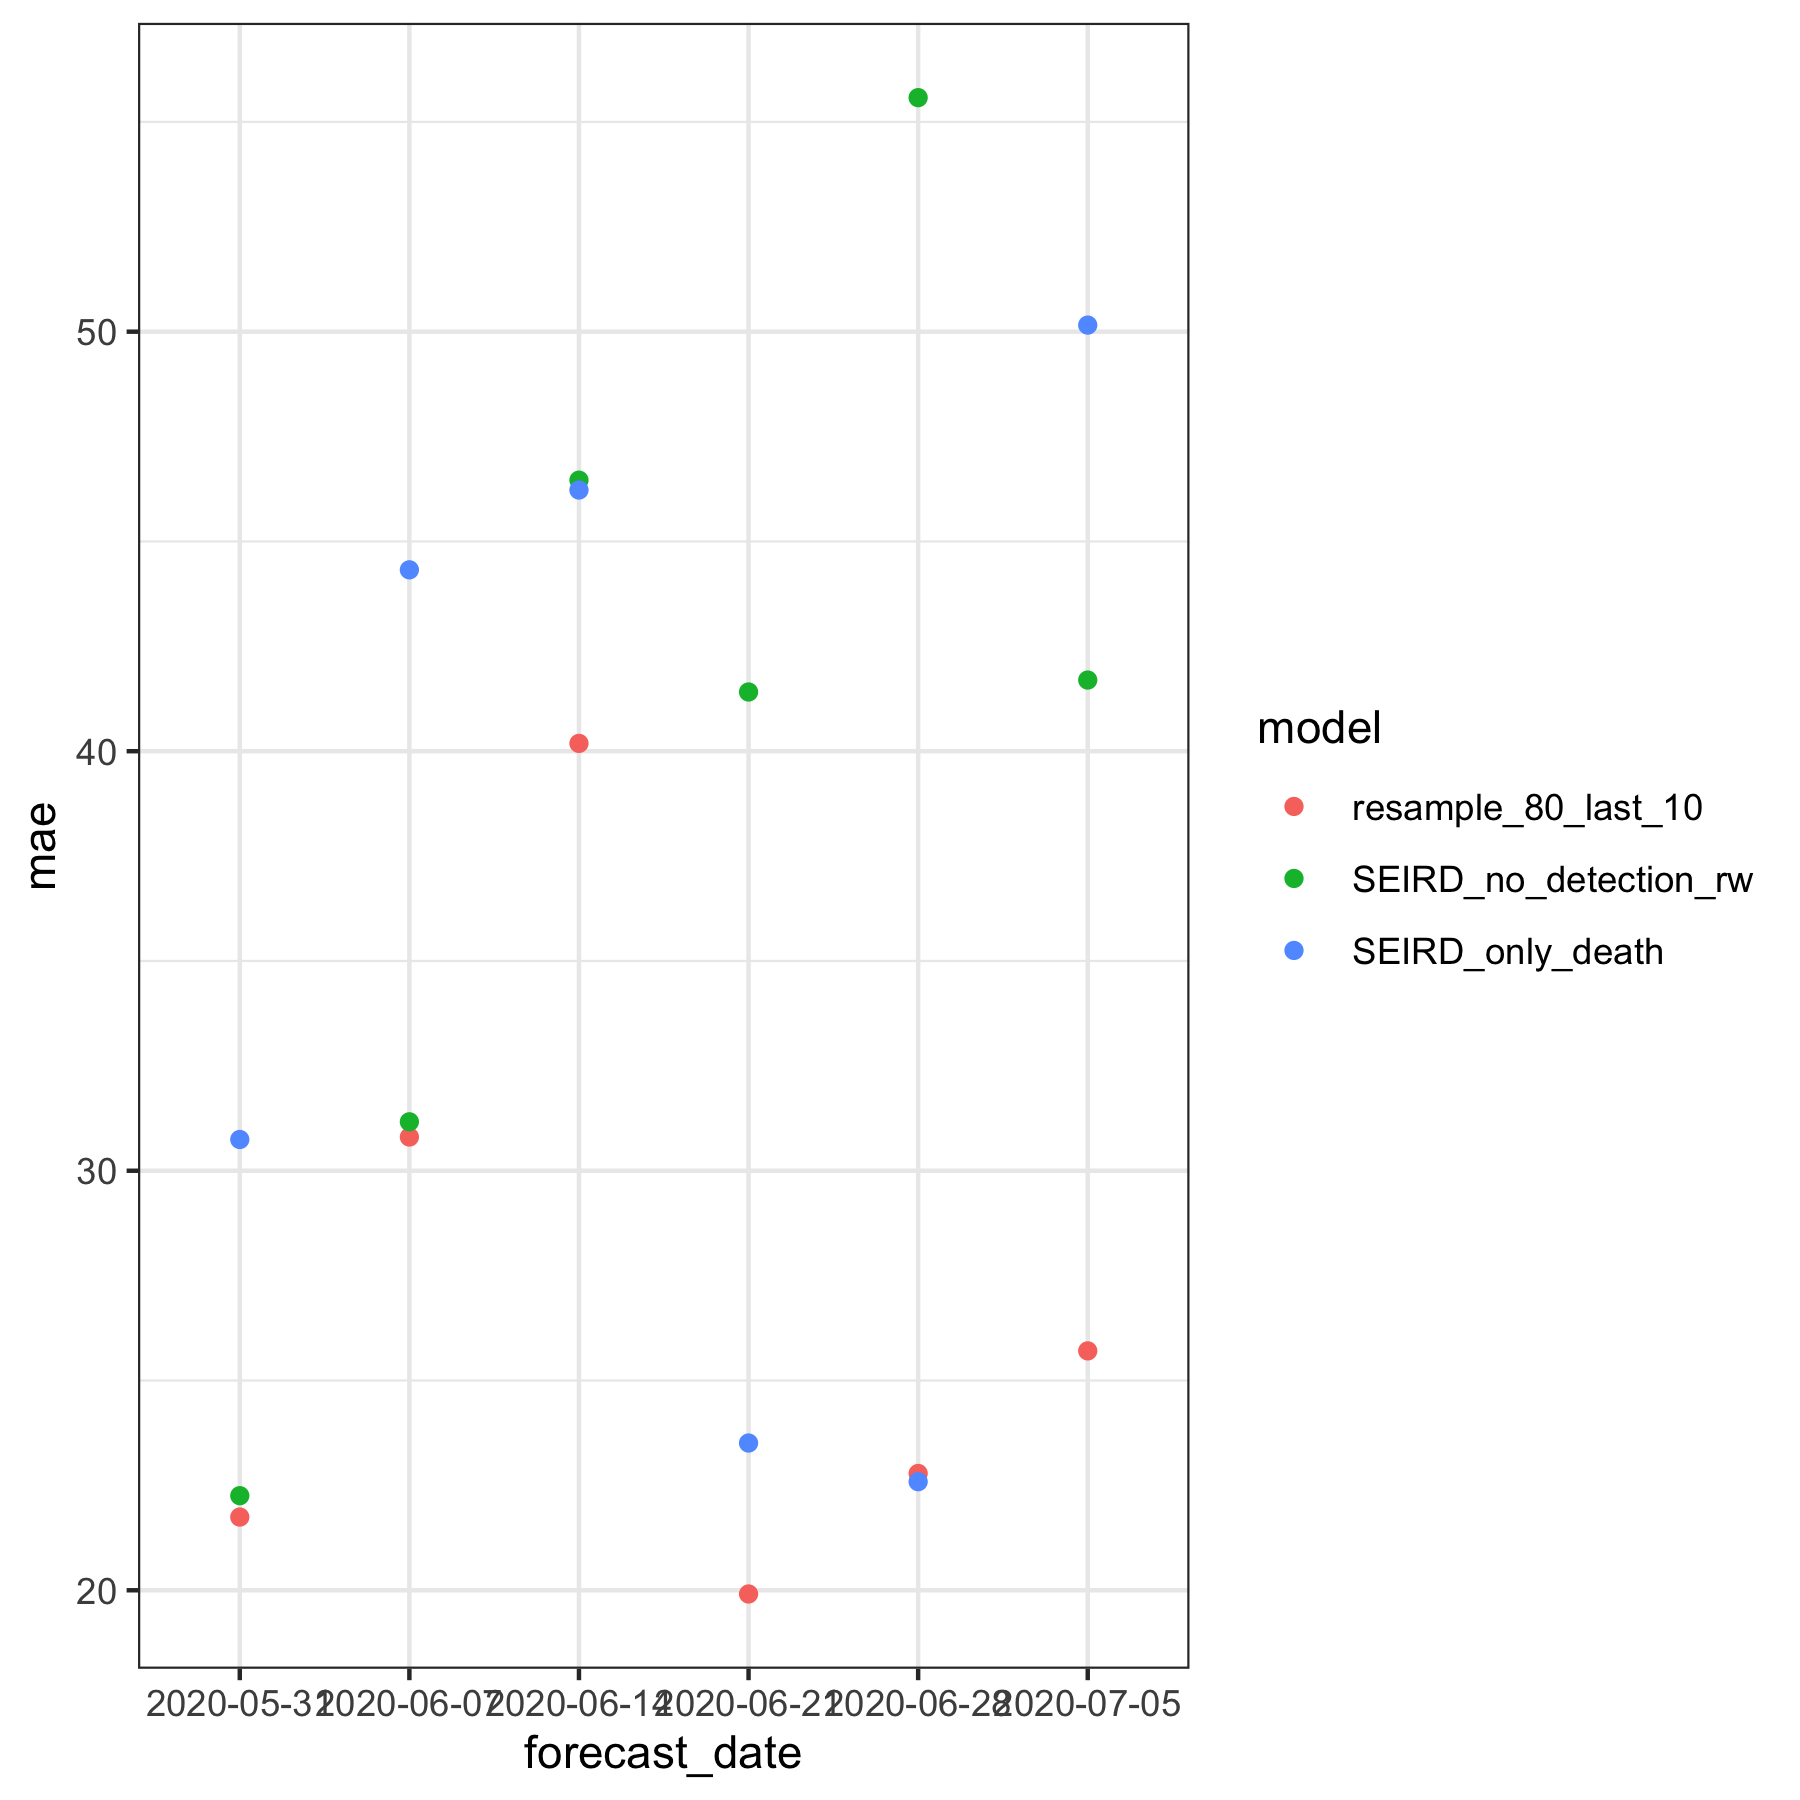
\includegraphics[scale=.15]{ablation_1.png}
    \caption{Ablation results for 1 week ahead.}
\end{subfigure}%
\begin{subfigure}{.5\textwidth}
  \centering
    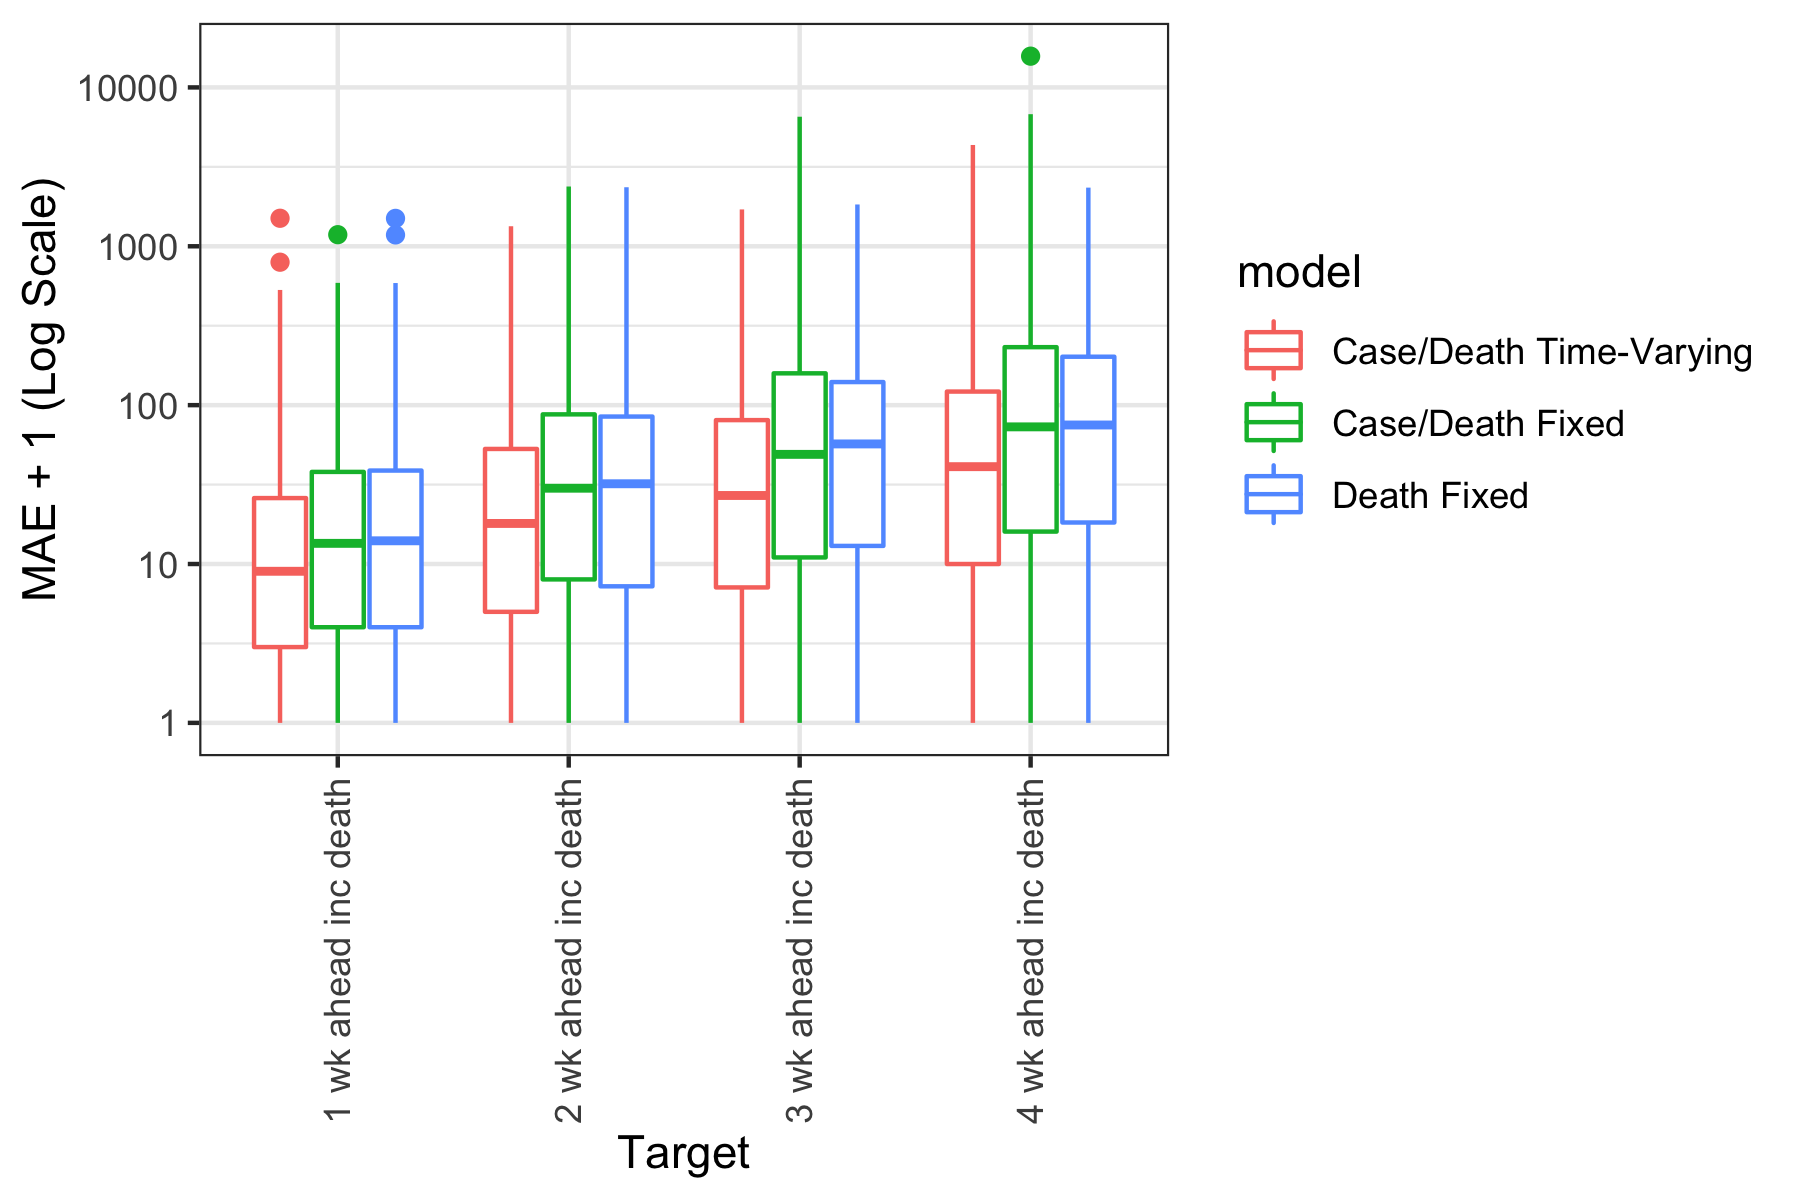
\includegraphics[scale=.15]{ablation_2.png}
    \caption{Ablation results for 2 week ahead.}
\end{subfigure}
\begin{subfigure}{.5\textwidth}
  \centering
    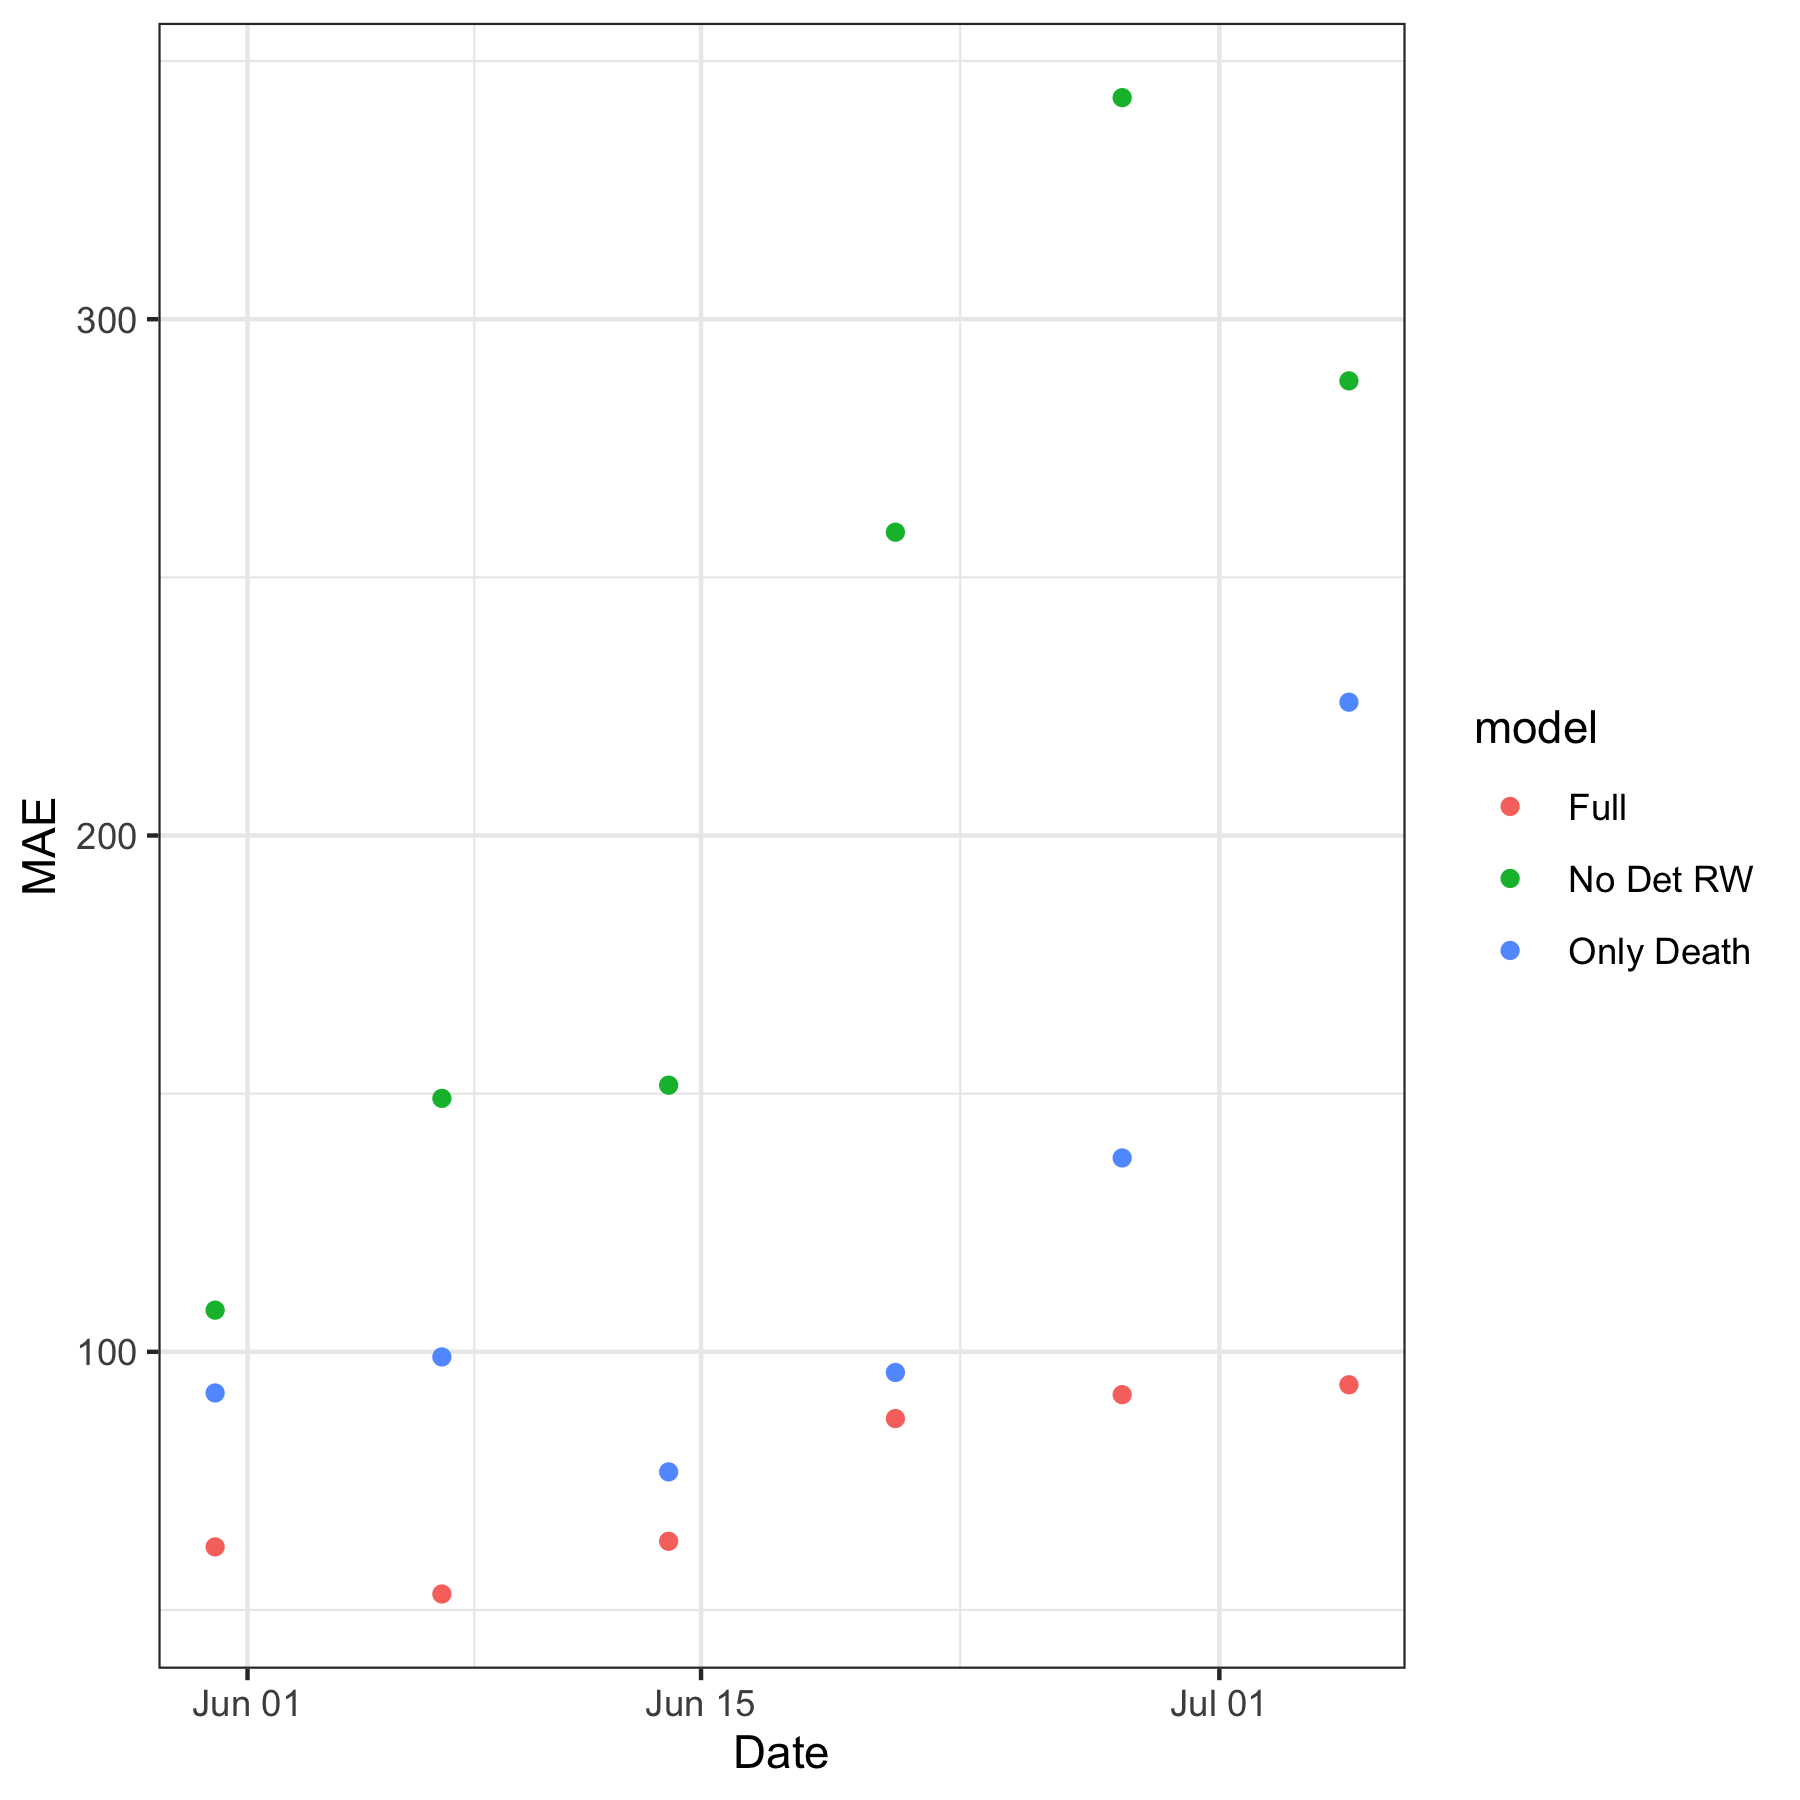
\includegraphics[scale=.15]{ablation_3.png}
    \caption{Ablation results 3 week ahead.}
\end{subfigure}%
\begin{subfigure}{.5\textwidth}
  \centering
    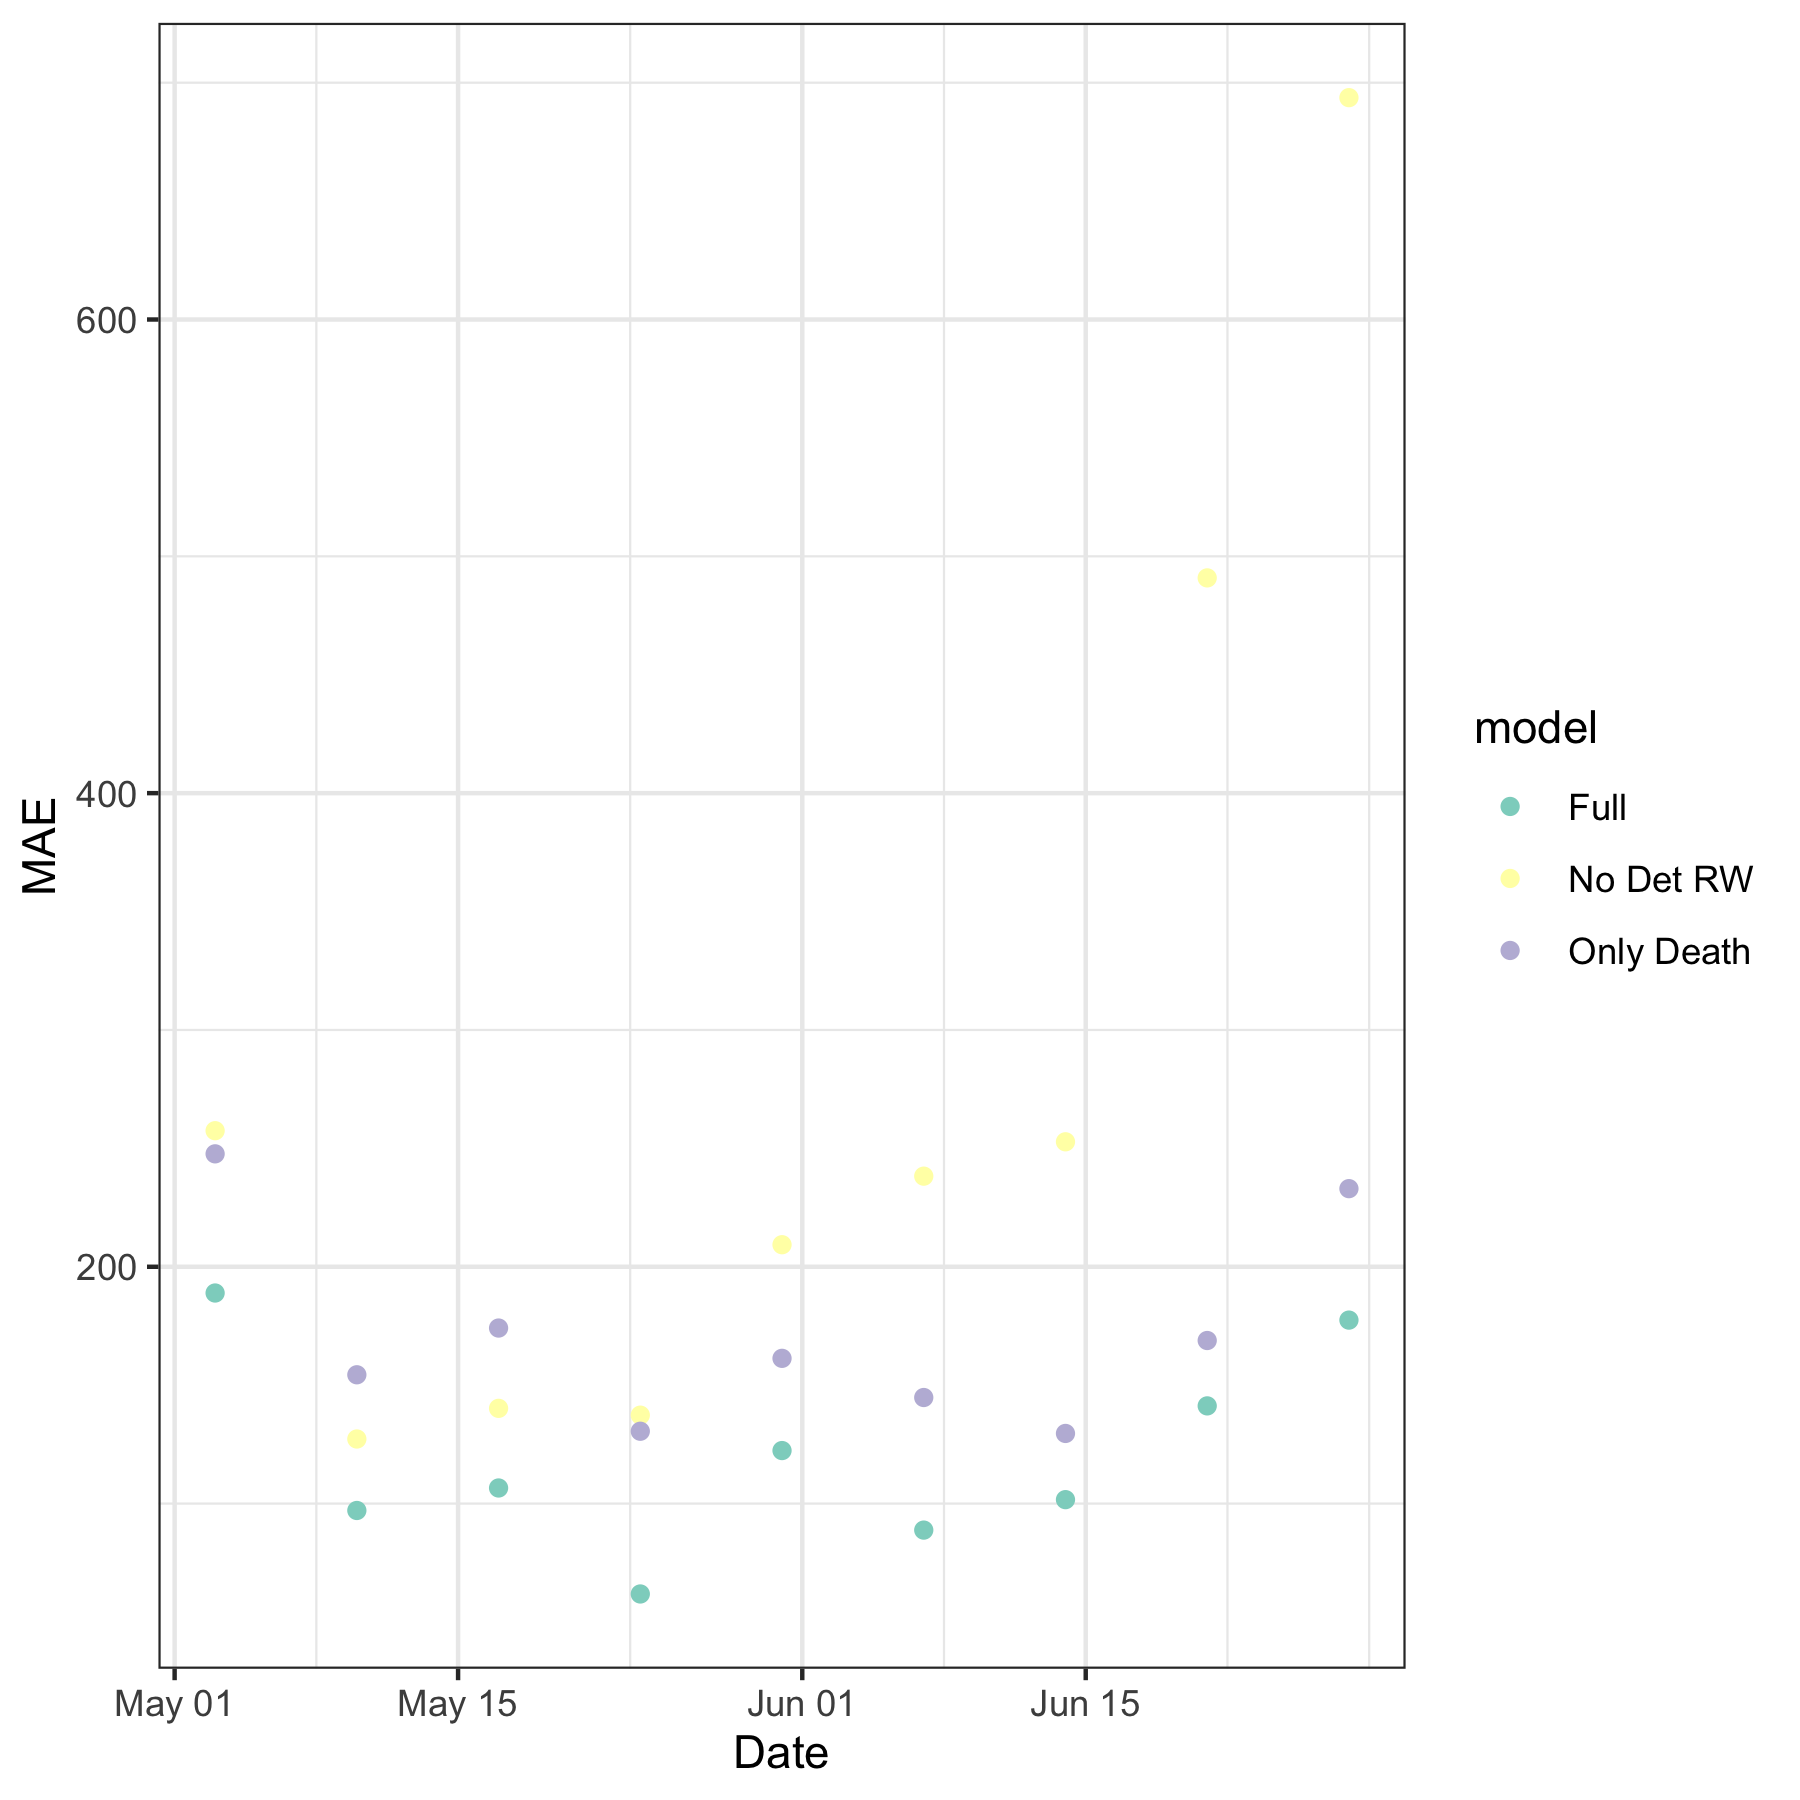
\includegraphics[scale=.15]{ablation_4.png}
    \caption{Ablation results 4 week ahead. }
\end{subfigure}

\caption{Scores from COVID-HUB broken down by region, target and timezero. Here we can see that the MechBayes model improves in both MAE and WIS over time, consistently beating the baseline model in the month of July 2020.  }
\label{fig:ablation}
\end{figure}




\section{Discussion}

MechBayes is a fast, fully Bayesian compartmental model capable of accounting for real-world modeling challenges during a pandemic. Our experiments led us to the following conclusions.

\begin{itemize}
\item \textbf{Adding case data when predicting deaths is helpful but only when accounting for data quality issues}. Our ablation test (Figure \ref{fig:ablation}) clearly shows that time-varying detection probability is a key feature in the model for reducing MAE of forecasts. As we can see in Figure \ref{fig:model_details}, the model relies on this parameter heavily, setting the detection probability at around 15\% at the start of the pandemic in March, to nearly 80\% by August 1st 2020. There is remarkable similarity between the increase across geographical locations as well, suggesting (as testing data reflects) an overall increase in the number of detected cases across the U.S. 

\item \textbf{Allowing for time-varying transmissibility is necessary to non-parametrically capture the effect of non-pharamceutical interventions}. Our ablation test explicitly did not include a model that fixed $\beta$ across time. This is because the model would not converge without the flexibility to capture interventions. While non-parametrically modeling interventions is appealing from a forecasting perspective, it does modify the philosophy behind compartmental modeling. By including such a flexible parameter, we may view MechBayes as simply a random-walk model, with a set of epidemiological parameters transforming that random-walk in an almost deterministic way to match both cases and deaths. For instance, if the variance of the random walk $\sigma_{\beta}^2$ was allowed to be arbitrarily large, then $\beta(t)$ could vary enough to match the data exactly. This would clearly attribute reporting issues as true changes in transmissibility. Bypassing the epidemiological interpretation that compartmental models provide. 

\item \textbf{Models must evolve in order to be successful in real-time pandemic forecasting}. As Figure \ref{fig:covidhub} shows, MechBayes significantly improved over time relative to the baseline model. Forecasting during a real-time pandemic is subject to a wide variety of data reporting issues. Continuously responding to challenges is key to being able to forecast well. 

\item \textbf{MechBayes is biased high}

\end{itemize}


\begin{figure}
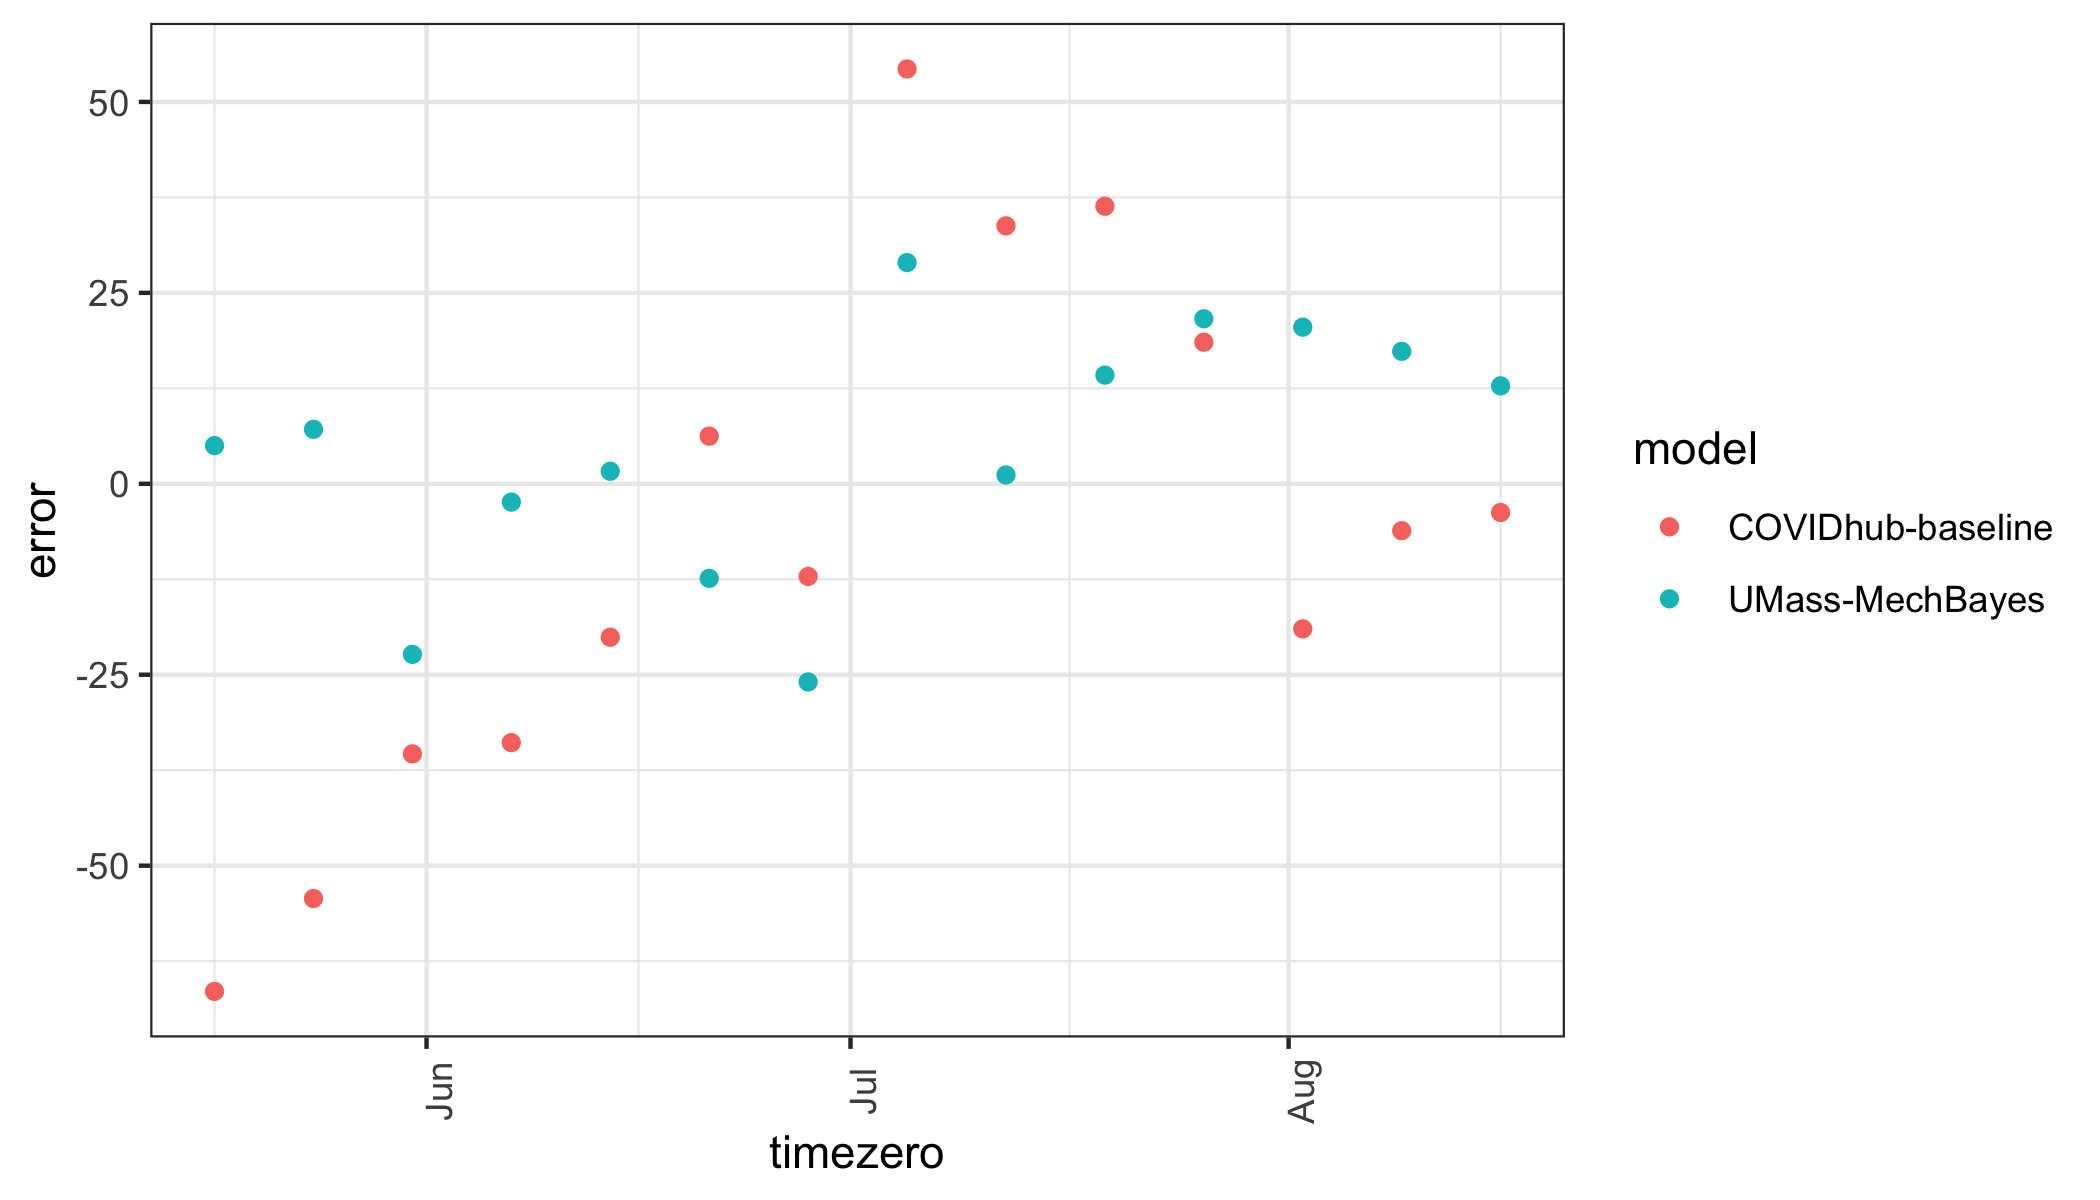
\includegraphics[scale=.2]{bias_by_timezero.png}

\caption{Bias of MechBayes and COVID-Baseline as a function of time..  }
\label{fig:bias}
\end{figure}


\section{Conclusion}

We have seen that MechBayes is a powerful Bayesian compartmental model that can capture the real-world complexities of forecasting during a pandemic. Through internal and external evaluation, we have demonstrated the success of MechBayes in forecasting. The model is able to improve over a naive baseline model as well as a naive compartmental model. Allowing for time-varying interventions and detection probability is a necessary model component during a real-time pandemic forecasting effort. 

While we chose an exponential random walk on $\beta(t)$ there are many other choices for flexible non-parametric modeling of transmissibility. Further work might consider a spline model, or a Gaussian process, or semi-parametric models capable of taking intervention dates as covariates. 

\newpage

\bibliographystyle{unsrt}
\bibliography{bib}

\end{document}  
